\documentclass[aspectratio=169]{ctexbeamer}

% ── 字体配置 ──
\setCJKmainfont{Noto Sans CJK SC}[
  BoldFont=Noto Sans CJK SC,
  ItalicFont=Noto Sans CJK SC
]
\setCJKsansfont{Noto Sans CJK SC}
\setCJKmonofont{Noto Sans Mono CJK SC}[
  ItalicFont=Noto Sans Mono CJK SC,
  BoldFont=Noto Sans Mono CJK SC
]

\usetheme{Madrid}
\usecolortheme{default}
\usepackage{tikz}
\usetikzlibrary{positioning, arrows.meta, calc, shapes.geometric}
\usepackage{booktabs}
\usepackage{listings}
\usepackage{graphicx}

\definecolor{mainblue}{RGB}{40,90,180}
\definecolor{lightblue}{RGB}{232,240,255}
\definecolor{redaccent}{RGB}{200,50,50}
\definecolor{greenaccent}{RGB}{40,140,60}
\definecolor{codebg}{RGB}{248,248,250}

\setbeamertemplate{navigation symbols}{}

\title{MNIST 手写数字识别：MLP 入门}
\subtitle{从感知机到多层神经网络——理论、直觉、代码三位一体}
\author{}
\date{}

\lstset{
  basicstyle=\ttfamily\small,
  keywordstyle=\color{mainblue}\bfseries,
  commentstyle=\color{greenaccent!50!black}\itshape,
  stringstyle=\color{redaccent},
  showstringspaces=false,
  breaklines=true,
  frame=single,
  rulecolor=\color{lightblue},
  backgroundcolor=\color{codebg},
  tabsize=4, language=Python,
  numbers=left, numberstyle=\tiny\color{gray}, numbersep=4pt,
  xleftmargin=0.3cm, framexleftmargin=0.3cm
}

\begin{document}

% ═══════════ 1 — 标题页 ═══════════
\begin{frame}
  \titlepage
  \vspace{-0.6cm}
  \begin{center}
    \large 核心问题：计算机如何从 $28\times 28$ 个像素中，识别一个手写数字？\\
    \normalsize 三个角度：\textbf{数学原理} $\to$ \textbf{直觉理解} $\to$ \textbf{Python 代码实现}
  \end{center}
\end{frame}

% ═══════════ 2 — 项目文件结构 ═══════════
\begin{frame}[shrink=15]{项目文件结构：四个模块各司其职}
\small

\begin{center}
\begin{tikzpicture}[
  node distance=0.3cm and 0.6cm,
  filebox/.style={draw, rounded corners, minimum width=3.6cm, minimum height=0.7cm,
                  align=center, font=\small},
  arrow/.style={->, >=stealth, thick, mainblue}, dep/.style={->, >=stealth, dashed, gray}
]
  \node[filebox, fill=lightblue!30] (data) {\textbf{data.py}\\数据加载模块};
  \node[filebox, fill=lightblue!40, right=of data] (utils) {\textbf{utils.py}\\工具函数模块};
  \node[filebox, fill=lightblue!50, below=of data] (models) {\textbf{models.py}\\模型定义模块};
  \node[filebox, fill=mainblue!25, below=of utils] (main) {\textbf{mnist\_mlp.py}\\主训练/测试脚本};
  \draw[dep] (main) -- (data);
  \draw[dep] (main) -- (utils);
  \draw[dep] (main) -- (models);
\end{tikzpicture}
\end{center}

\vspace{0.15cm}

\begin{columns}[T]
\column{0.5\textwidth}
\footnotesize
\begin{block}{\texttt{data.py} + \texttt{utils.py}}
\begin{itemize}
  \item \texttt{get\_mnist\_loaders()}：下载 MNIST、ToTensor 归一化、构造 DataLoader
  \item \texttt{get\_device()}：自动选 GPU/CPU
  \item \texttt{set\_seed()}：固定随机种子（保证可复现）
  \item \texttt{accuracy()}：计算分类准确率
  \item \texttt{save\_checkpoint()}：保存模型参数
\end{itemize}
\end{block}

\column{0.5\textwidth}
\footnotesize
\begin{block}{\texttt{models.py} + \texttt{mnist\_mlp.py}}
\begin{itemize}
  \item \texttt{MLPClassifier}：784$\to$128$\to$64$\to$10 (Flatten+Linear+ReLU)
  \item \texttt{train\_one\_epoch()}：训练循环（5 个核心步骤）
  \item \texttt{evaluate()}：测试评估（eval + no\_grad）
  \item \texttt{main()}：串联完整流程，保存 checkpoint
\end{itemize}
\end{block}
\end{columns}
\end{frame}

% ═══════════ 3 — MNIST 数据集 + data.py + 手写图 ═══════════
\begin{frame}[fragile,shrink=15]{MNIST 数据集：先看看我们要识别的图片}
\footnotesize

\begin{columns}[T]
\column{0.38\textwidth}
\begin{center}
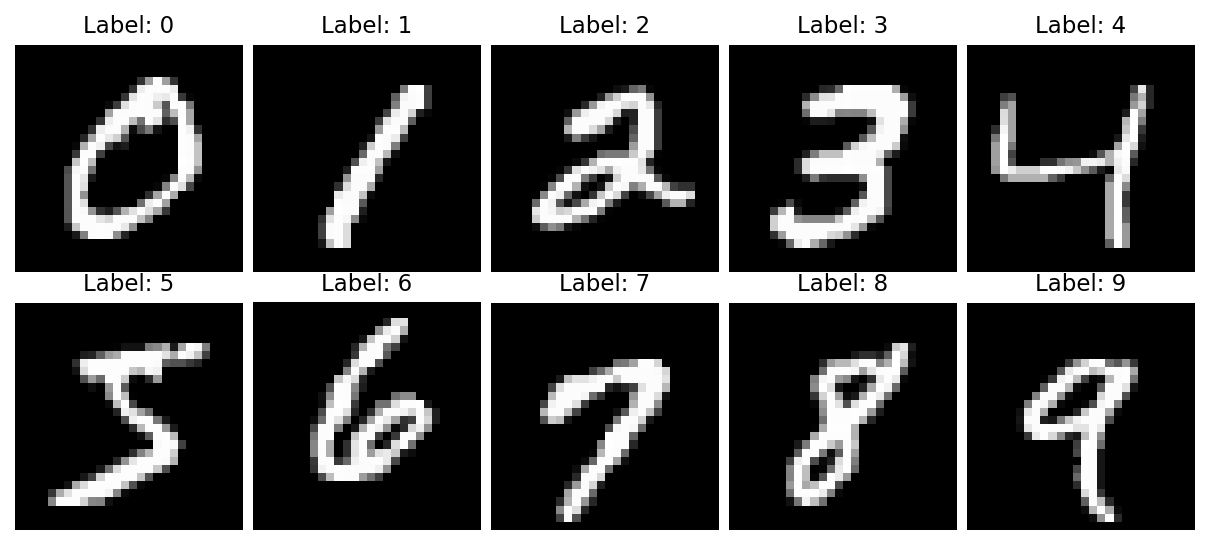
\includegraphics[width=\textwidth]{slide_assets/mnist_samples.png}
\end{center}
\vspace{-0.3cm}
\begin{center}
\scriptsize 训练集 60,000 张 + 测试集 10,000 张，28$\times$28 灰度图，10 个类别
\end{center}

\column{0.62\textwidth}
\begin{block}{\texttt{data.py} — 数据如何变成张量}
\begin{lstlisting}[basicstyle=\ttfamily\scriptsize, frame=none, numbers=none, backgroundcolor=\color{codebg}]
transform = transforms.ToTensor()
train_data = datasets.MNIST(
    root="datasets", train=True,
    download=True, transform=transform)
train_loader = DataLoader(train_data,
    batch_size=64, shuffle=True)
\end{lstlisting}
\end{block}

\vspace{0.15cm}

\begin{block}{一张图如何进入神经网络？}
\begin{center}
\begin{tikzpicture}[scale=0.85, node distance=0.6cm]
  \node[font=\footnotesize] (raw) {28$\times$28 像素矩阵};
  \node[font=\footnotesize, right=of raw] (t) {\texttt{ToTensor()}};
  \node[font=\footnotesize, right=of t] (flat) {784 维向量};
  \node[font=\footnotesize, right=of flat] (net) {MLP 网络};
  \draw[->, thick, mainblue] (raw) -- (t);
  \draw[->, thick, mainblue] (t) -- (flat);
  \draw[->, thick, mainblue] (flat) -- (net);
\end{tikzpicture}
\end{center}
\vspace{-0.2cm}
每个像素是一个输入神经元，784 个像素值就是 784 个输入。\\[2pt]
\textbf{关键：} \texttt{shuffle=True} 训练时打乱顺序；\texttt{shuffle=False} 测试时保持顺序。
\end{block}
\end{columns}
\end{frame}

% ═══════════ 4 — MLP 架构 + models.py ═══════════
\begin{frame}[fragile,shrink=15]{MLP 网络结构：\texttt{models.py} 中的 \texttt{MLPClassifier}}
\small

\begin{columns}[T]
\column{0.45\textwidth}
\begin{center}
\begin{tikzpicture}[scale=0.78,
  neuron/.style={circle, draw, minimum size=0.32cm, inner sep=0pt, fill=lightblue!60},
  arrow/.style={->, >=stealth, thick, mainblue}
]
  \foreach \i in {1,...,6}
    \node[neuron] (I\i) at (0, 0.9*\i-3.15) {};
  \node[font=\tiny] at (0, -3.7) {输入 784};

  \foreach \i in {1,...,5}
    \node[neuron] (H\i) at (2.2, 0.9*\i-2.7) {};
  \node[font=\tiny] at (2.2, -3.7) {隐藏1 128};

  \foreach \i in {1,...,4}
    \node[neuron] (H2\i) at (4.2, 0.9*\i-2.25) {};
  \node[font=\tiny] at (4.2, -3.7) {隐藏2 64};

  \foreach \i in {1,...,5}
    \node[neuron] (O\i) at (6.2, 0.9*\i-2.7) {};
  \node[font=\tiny] at (6.2, -3.7) {输出 10};

  \foreach \i in {1,...,6}
    \foreach \j in {1,...,5}
      \draw[arrow, opacity=0.08] (I\i) -- (H\j);
  \foreach \i in {1,...,5}
    \foreach \j in {1,...,4}
      \draw[arrow, opacity=0.08] (H\i) -- (H2\j);
  \foreach \i in {1,...,4}
    \foreach \j in {1,...,5}
      \draw[arrow, opacity=0.08] (H2\i) -- (O\j);
\end{tikzpicture}
\end{center}
\vspace{-0.3cm}
\begin{table}
\footnotesize
\begin{tabular}{l r}
\toprule
\textbf{层} & \textbf{参数量} \\
\midrule
Linear(784$\to$128) & 100,480 \\
Linear(128$\to$64)  & 8,256   \\
Linear(64$\to$10)   & 650     \\
\midrule
\textbf{总计}       & \textbf{109,386} \\
\bottomrule
\end{tabular}
\end{table}

\column{0.55\textwidth}
\begin{block}{\texttt{models.py} 完整代码}
\footnotesize
\begin{lstlisting}[basicstyle=\ttfamily\scriptsize, frame=none, numbers=none, backgroundcolor=\color{codebg}]
class MLPClassifier(nn.Module):
    def __init__(self):
        super().__init__()
        self.net = nn.Sequential(
            nn.Flatten(),        # (a)
            nn.Linear(784, 128), # (b)
            nn.ReLU(),           # (c)
            nn.Linear(128, 64),  # (d)
            nn.ReLU(),           # (e)
            nn.Linear(64, 10),   # (f)
        )
    def forward(self, x):
        return self.net(x)       # (g)
\end{lstlisting}
\end{block}
\vspace{0.1cm}
\footnotesize
\textbf{标注对应后面各页详解：}
\begin{itemize}
  \item (a) Flatten：把图像"拉直"成一维向量
  \item (b)(d)(f) Linear：矩阵乘法 $y=Wx+b$，共 3 层
  \item (c)(e) ReLU：$\max(0,x)$，引入非线性
  \item (g) forward：一行代码完成全部前向计算
\end{itemize}
\end{columns}
\end{frame}

% ═══════════ 5 — Flatten + Linear + ReLU 直观解释 ═══════════
\begin{frame}[shrink=15]{从像素到特征：Flatten、Linear、ReLU 各做了什么}
\small

\begin{columns}[T]
\column{0.33\textwidth}
\begin{block}{Flatten（\texttt{models.py} (a)）}
\begin{center}
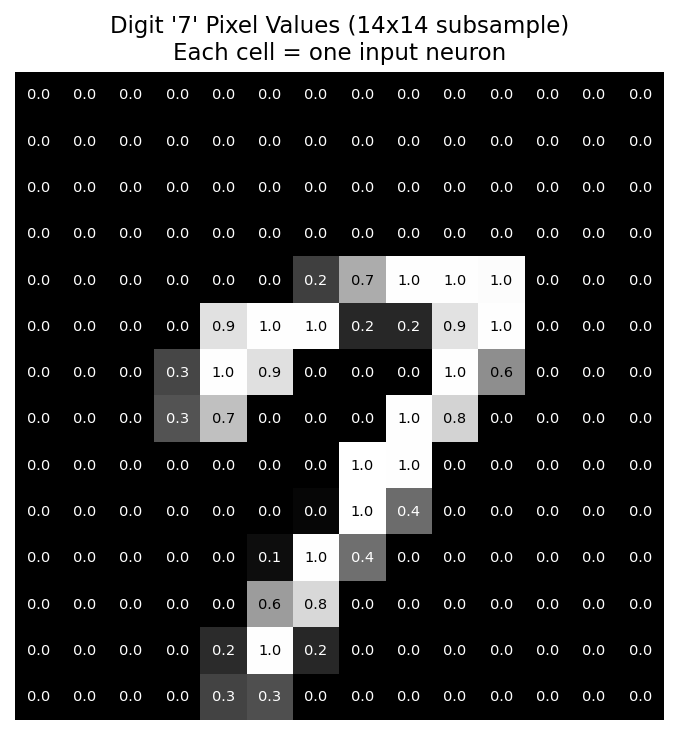
\includegraphics[width=2.5cm]{slide_assets/digit_grid.png}
\end{center}
\vspace{-0.3cm}
\footnotesize
把 28$\times$28 的矩阵\\
"拉直"成一维向量。\\
\textbf{不改变数值}，\\
只是重新排列。

\textbf{代价：}丢弃像素间的\\
空间位置关系。这正是\\
MLP 与 CNN 的核心区别。
\end{block}

\column{0.33\textwidth}
\begin{block}{Linear（\texttt{models.py} (b)(d)(f)）}
\footnotesize
\[
y = Wx + b
\]

\vspace{-0.2cm}
每个 Linear 层是一个\\
"特征检测器"。

$W$ 的每一行 = 一个\\
"模式模板"：\\
\hspace{4pt}$w_{ij}>0$：像素 $j$ 推高输出 $i$\\
\hspace{4pt}$w_{ij}<0$：像素 $j$ 拉低输出 $i$

$b$：允许输出整体平移。
\end{block}

\column{0.34\textwidth}
\begin{block}{ReLU（\texttt{models.py} (c)(e)）}
\footnotesize
\[
f(x) = \max(0, x)
\]
\begin{center}
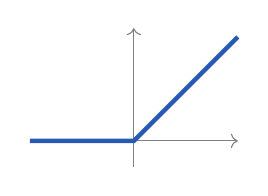
\begin{tikzpicture}[scale=1.1]
  \draw[->, gray] (-1.2,0) -- (1.2,0);
  \draw[->, gray] (0,-0.3) -- (0,1.3);
  \draw[ultra thick, mainblue] (-1.2,0) -- (0,0) -- (1.2,1.2);
\end{tikzpicture}
\end{center}
\vspace{-0.3cm}
\textbf{为什么必须？}\\
没有 ReLU，两层 Linear\\
等价于一层：\\
$W_2(W_1 x+b_1)+b_2$\\
$=W'x + b'$

ReLU 打破"线性坍缩"。
\end{block}
\end{columns}
\end{frame}

% ═══════════ 6 — Softmax 直观解释 ═══════════
\begin{frame}[shrink=25]{Softmax：把原始分数变成概率分布}
\small

\begin{columns}[T]
\column{0.48\textwidth}
\begin{center}
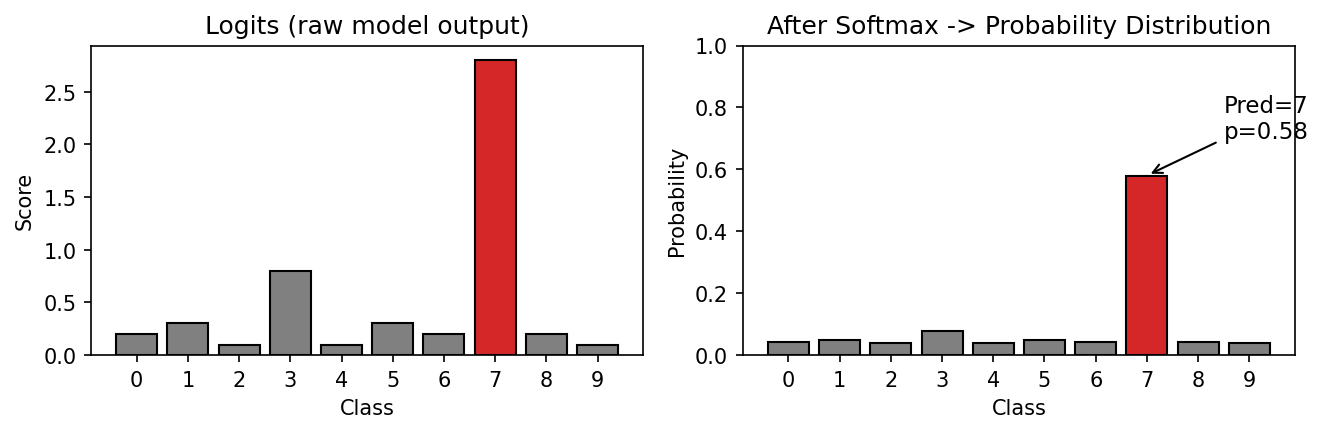
\includegraphics[width=\textwidth]{slide_assets/softmax_viz.png}
\end{center}
\vspace{-0.2cm}
\begin{exampleblock}{如何读左图？}
\footnotesize
\textbf{左图 Logits：} 模型原始输出，可正可负，数值范围不固定。类别 7 的分数 2.8 最高，但难以直观判断"有多大把握"。\\[2pt]
\textbf{右图 Softmax 后：} 转为概率——类别 7 概率约 0.62，其余 9 类合计约 0.38。一眼看出模型对"7"有 62\% 把握。\\[2pt]
\textbf{指数 $e^{z_i}$ 的效果：} 放大高分、缩小低分，让最大 logit 在概率中\"脱颖而出\"。
\end{exampleblock}

\column{0.52\textwidth}
\begin{block}{Softmax 做了什么？}
\footnotesize
模型输出 10 个 \textbf{logits}（原始分数，可正可负）。Softmax 把它变成概率分布（非负、和为 1）：
\[
p_i = \frac{e^{z_i}}{\sum_{j=0}^{9} e^{z_j}}
\]
\end{block}

\vspace{0.1cm}

\begin{exampleblock}{直观类比}
\footnotesize
Logits = 评委打分，Softmax = 按分数分配获奖概率。\\
分数最高者概率最高，但其他人也有机会。
\end{exampleblock}

\vspace{0.1cm}

\footnotesize
\textbf{为何模型里不加 Softmax？} CrossEntropyLoss 内部已包含。\\[1pt]
\textbf{代码：} \texttt{models.py} Linear(64,10) 出 logits，\texttt{mnist\_mlp.py:74} CrossEntropyLoss 自动做 Softmax。
\end{columns}
\end{frame}

% ═══════════ 7 — 交叉熵损失直观解释 ═══════════
\begin{frame}[fragile,shrink=15]{交叉熵损失 (CrossEntropyLoss)：量化"预测有多偏离正确答案"}
\small

\begin{center}
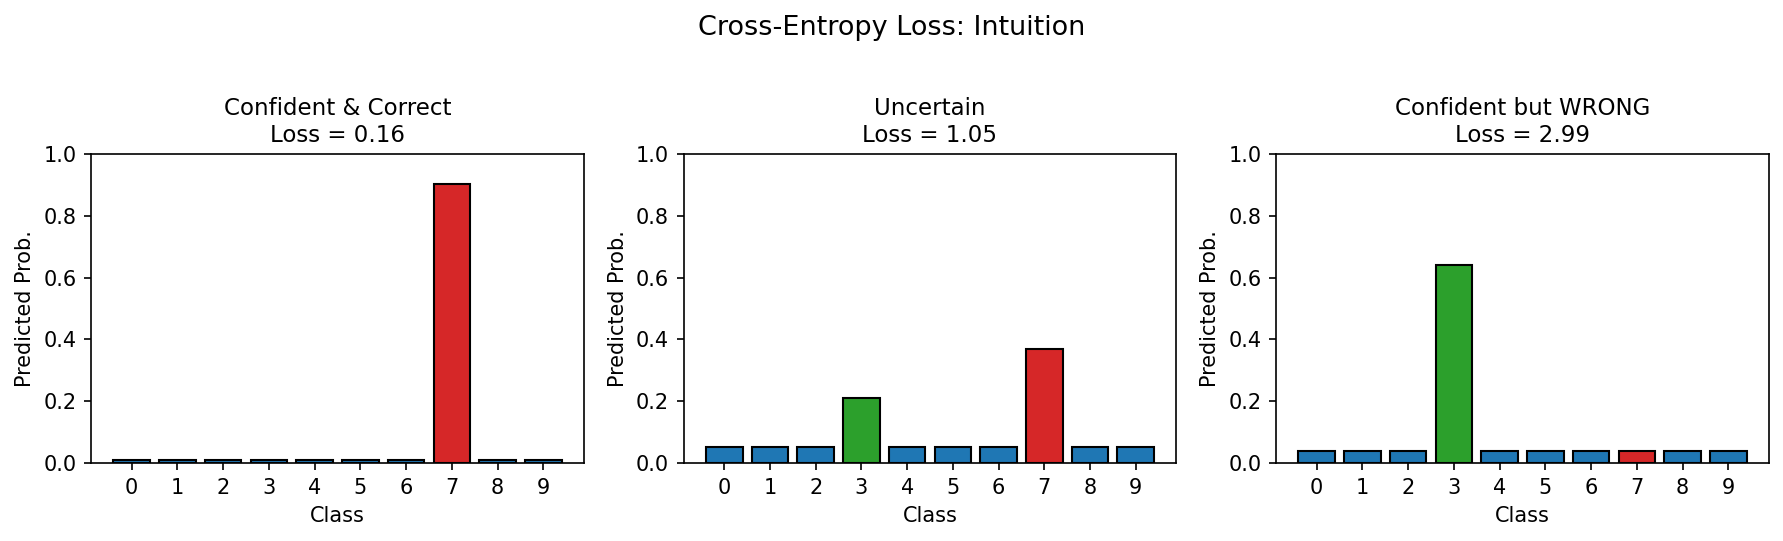
\includegraphics[width=0.85\textwidth]{slide_assets/crossentropy_viz.png}
\end{center}

\vspace{0.15cm}

\begin{columns}[T]
\column{0.5\textwidth}
\begin{block}{数学定义（\texttt{mnist\_mlp.py:74}）}
\footnotesize
\begin{lstlisting}[basicstyle=\ttfamily\footnotesize, frame=none, numbers=none, backgroundcolor=\color{codebg}]
criterion = nn.CrossEntropyLoss()
\end{lstlisting}
内部两步：\\[2pt]
1. \textbf{Softmax}：$p_i = e^{z_i} / \sum e^{z_j}$\\[2pt]
2. \textbf{负对数似然}：
   $\text{Loss} = -\ln(p_{\text{true}})$
\end{block}

\column{0.5\textwidth}
\begin{exampleblock}{直观理解：三个场景}
\footnotesize
\textbf{场景 1 (Loss=0.16)：} 模型很确信，而且对了——Loss 很小。

\textbf{场景 2 (Loss=1.05)：} 模型不太确定，概率分散到几个类别——Loss 中等。

\textbf{场景 3 (Loss=2.99)：} 模型非常确信一个错误的答案——Loss 最大，这是最糟糕的情况！
\end{exampleblock}
\end{columns}

\vspace{0.15cm}
\footnotesize
\textbf{在训练循环中：} \texttt{mnist\_mlp.py:29} 的 \texttt{loss = criterion(logits, targets)} 计算的就是这个值。
\end{frame}

% ═══════════ 8 — 前向传播 ═══════════
\begin{frame}[fragile,shrink=20]{前向传播：数据在 4 个文件中如何流转}
\small

\begin{center}
\begin{tikzpicture}[
  node distance=0.3cm and 0.3cm,
  block/.style={draw, rounded corners, minimum width=2.0cm, minimum height=0.65cm,
                align=center, font=\footnotesize},
  arrow/.style={->, >=stealth, thick, mainblue}
]
  \node[block, fill=lightblue!40] (a) {\texttt{[64,1,28,28]}\\输入 batch};
  \node[block, fill=lightblue!50, right=of a] (b) {\texttt{[64,784]}\\Flatten};
  \node[block, fill=lightblue!60, right=of b] (c) {\texttt{[64,128]}\\Linear+ReLU};
  \node[block, fill=lightblue!70, right=of c] (d) {\texttt{[64,64]}\\Linear+ReLU};
  \node[block, fill=mainblue!25, right=of d] (e) {\texttt{[64,10]}\\输出 logits};
  \draw[arrow] (a) -- (b);
  \draw[arrow] (b) -- (c);
  \draw[arrow] (c) -- (d);
  \draw[arrow] (d) -- (e);
\end{tikzpicture}
\end{center}

\vspace{0.1cm}

\begin{columns}[T]
\column{0.48\textwidth}
\begin{block}{涉及的文件和代码行}
\footnotesize
\begin{itemize}
  \item \texttt{data.py:19-24} DataLoader 产出 (images, targets)
  \item \texttt{models.py:16-17} \texttt{forward(self, x): return self.net(x)}
  \item \texttt{mnist\_mlp.py:28} 训练中: \texttt{logits = model(images)}
  \item \texttt{mnist\_mlp.py:50} 测试中: \texttt{logits = model(images)}
\end{itemize}
\textbf{训练和测试的前向传播完全一样！}
\end{block}

\column{0.52\textwidth}
\begin{block}{数学表达}
\footnotesize
\[
\text{logits} = W_3 \cdot \text{ReLU}(W_2 \cdot \text{ReLU}(W_1 \cdot
\underbrace{\text{flatten}(x)}_{784} + b_1) + b_2) + b_3
\]

整个计算是\textbf{确定性的}：\\
固定输入 + 固定参数 = 固定输出。\\[2pt]
\textbf{不需要 PyTorch，不需要梯度。}\\
$\to$ 为 Python 训练 $\to$ C 推理创造了条件。
\end{block}
\end{columns}
\end{frame}

% ═══════════ 9 — 训练循环核心 5 步 ═══════════
\begin{frame}[fragile,shrink=20]{训练循环：\texttt{mnist\_mlp.py} 中 \texttt{train\_one\_epoch} 的 5 个步骤}
\footnotesize

\begin{block}{核心代码（\texttt{mnist\_mlp.py:24--31}）}
\begin{lstlisting}[basicstyle=\ttfamily\small, frame=single, backgroundcolor=\color{codebg}]
for images, targets in train_loader:
    images, targets = images.to(device), targets.to(device)

    optimizer.zero_grad()                  # 1. 清空累积的梯度
    logits = model(images)                 # 2. 前向传播 → 预测分数
    loss = criterion(logits, targets)      # 3. 计算损失
    loss.backward()                        # 4. 反向传播 → 计算梯度
    optimizer.step()                       # 5. 参数更新 → 梯度下降
\end{lstlisting}
\end{block}

\vspace{0.15cm}

\begin{center}
\begin{tikzpicture}[
  node distance=0.3cm,
  stepbox/.style={draw, rounded corners, minimum width=2.0cm, minimum height=0.55cm,
                  align=center, font=\footnotesize, fill=lightblue!60}
]
  \node[stepbox] (a) {1. zero\_grad()};
  \node[stepbox, right=of a] (b) {2. model(x)};
  \node[stepbox, right=of b] (c) {3. criterion()};
  \node[stepbox, right=of c] (d) {4. backward()};
  \node[stepbox, right=of d] (e) {5. step()};
  \draw[->, >=stealth, thick, mainblue] (a) -- (b);
  \draw[->, >=stealth, thick, mainblue] (b) -- (c);
  \draw[->, >=stealth, thick, mainblue] (c) -- (d);
  \draw[->, >=stealth, thick, mainblue] (d) -- (e);
  \draw[->, >=stealth, thick, mainblue, bend left=35] (e.south) to (a.south);
  \node[font=\footnotesize] at (6.5, -1.2) {每个 batch 重复一次};
\end{tikzpicture}
\end{center}

\vspace{0.1cm}
\footnotesize
\textbf{所有监督学习的训练循环都是这 5 步。} CNN、Transformer、GPT —— 无一例外。区别只在于第 2. 步中的 \texttt{model} 内部结构不同。
\end{frame}

% ═══════════ 10 — 反向传播 + 梯度下降 ═══════════
\begin{frame}[fragile,shrink=15]{梯度下降：模型如何"学习"——在损失平面上寻找最低点}
\small

\begin{columns}[T]
\column{0.5\textwidth}
\begin{center}
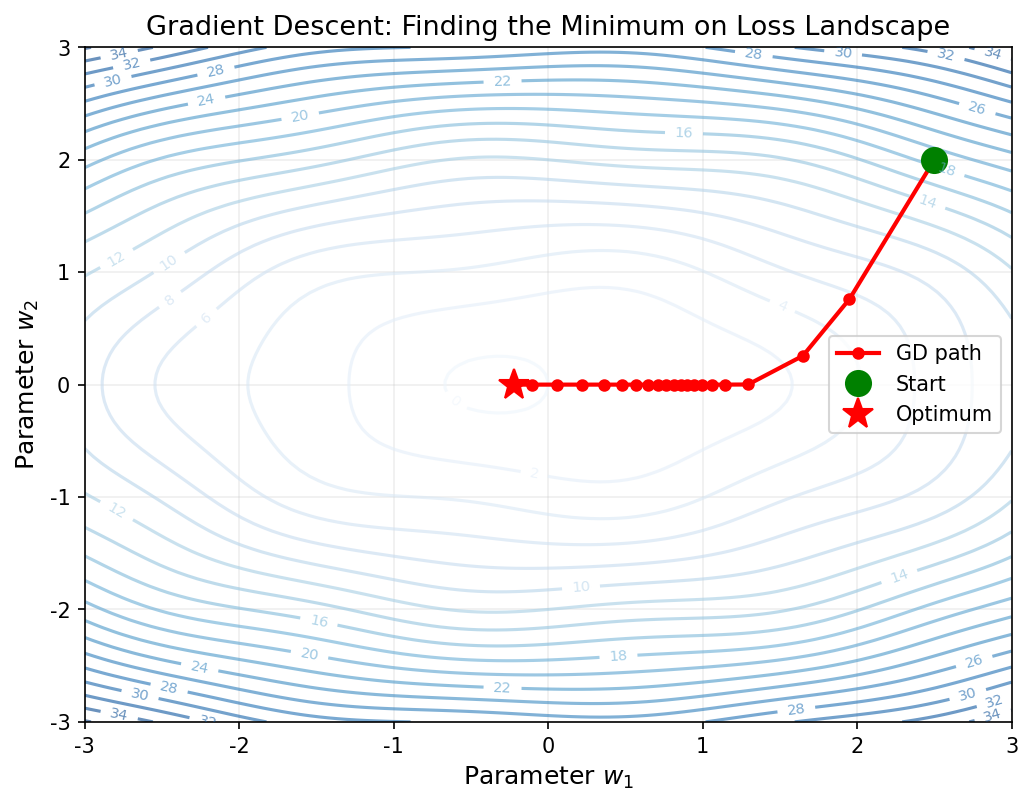
\includegraphics[width=\textwidth]{slide_assets/gd_landscape.png}
\end{center}

\column{0.5\textwidth}
\begin{block}{反向传播（\texttt{mnist\_mlp.py:30}）}
\footnotesize
\texttt{loss.backward()} 自动计算每个参数的梯度：
\[
\frac{\partial L}{\partial w} \quad\text{对所有 } w
\]
从损失出发，沿计算图反向逐层用链式法则求偏导数。这就是 PyTorch \textbf{autograd} 的核心。
\end{block}

\vspace{0.15cm}

\begin{block}{梯度下降（\texttt{mnist\_mlp.py:31 + :75}）}
\footnotesize
\texttt{optimizer.step()} 沿梯度负方向更新参数：
\[
w_{\text{new}} = w_{\text{old}} - \eta \cdot \frac{\partial L}{\partial w}
\]
\begin{lstlisting}[basicstyle=\ttfamily\footnotesize, frame=none, numbers=none, backgroundcolor=\color{codebg}]
optimizer = torch.optim.Adam(
    model.parameters(), lr=1e-3)
\end{lstlisting}
\textbf{Adam} = Momentum + RMSprop，自适应调整学习率。
\end{block}
\end{columns}

\vspace{0.15cm}
\footnotesize
\textbf{直观理解：} 想象你站在山顶（初始参数）要找最低点。你看一眼脚下的坡度（梯度），往最陡的下坡方向走一小步（步长 = 学习率 $\eta$）。重复这个过程，直到到达谷底。这就是梯度下降。
\end{frame}

% ═══════════ 11 — SGD vs Batch GD vs Mini-batch ═══════════
\begin{frame}[shrink=25]{梯度下降的三种变体：Batch GD vs SGD vs Mini-batch GD}
\small

\begin{center}
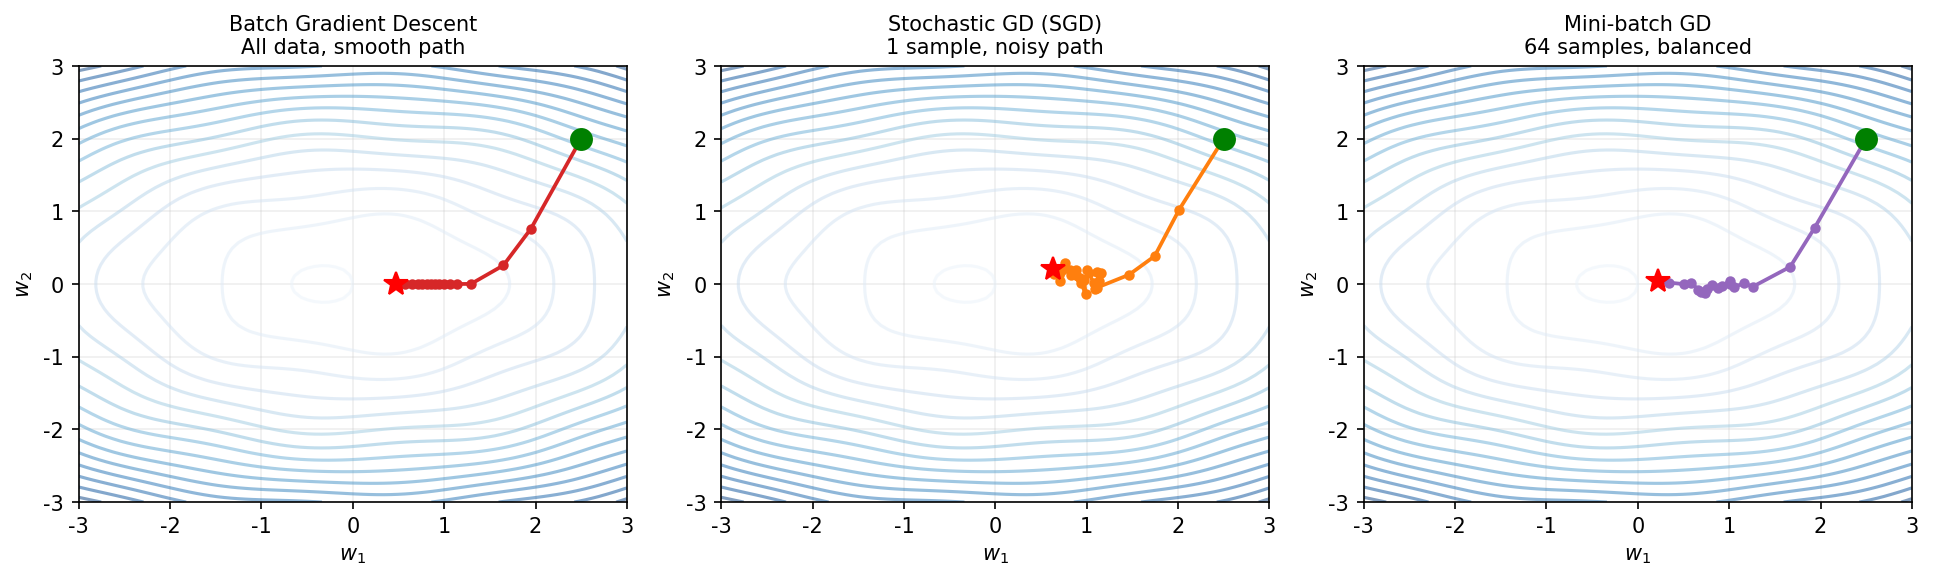
\includegraphics[width=0.88\textwidth]{slide_assets/gd_comparison.png}
\end{center}

\vspace{0.05cm}

\begin{columns}[T]
\column{0.33\textwidth}
\begin{block}{Batch GD（全量）}
\footnotesize
每次用全部 60,000 张图计算梯度。\\
\textbf{优点：} 梯度精确，路径平滑。\\
\textbf{缺点：} 每步太慢，显存放不下大数据集。
\end{block}

\column{0.33\textwidth}
\begin{block}{SGD（随机）}
\footnotesize
每次只用 1 张图。\\
\textbf{优点：} 极快，可跳出局部最优。\\
\textbf{缺点：} 噪声大，路径震荡。
\end{block}

\column{0.34\textwidth}
\begin{block}{Mini-batch GD（本实验用）}
\footnotesize
每次 64 张图（\texttt{data.py} \texttt{batch\_size}）。\\
\textbf{优点：} 兼顾速度和稳定性，GPU 并行高效。\\[1pt]
\textit{大多数深度学习都用 Mini-batch GD。}
\end{block}
\end{columns}
\end{frame}

% ═══════════ 12 — 训练 vs 测试 ═══════════
\begin{frame}[fragile,shrink=15]{训练 vs 测试：\texttt{train\_one\_epoch} 与 \texttt{evaluate} 的对比}
\small

\begin{columns}[T]
\column{0.48\textwidth}
\begin{block}{\texttt{train\_one\_epoch}（\texttt{mnist\_mlp.py:12--36}）}
\footnotesize
\begin{lstlisting}[basicstyle=\ttfamily\footnotesize, frame=none, numbers=none, backgroundcolor=\color{codebg}]
model.train()          # 训练模式
for images, targets in loader:
    optimizer.zero_grad()
    logits = model(images)
    loss = criterion(logits, targets)
    loss.backward()     # 计算梯度
    optimizer.step()    # 更新参数
\end{lstlisting}
\alert{参数会改变！模型在"学习"。}
\end{block}

\column{0.52\textwidth}
\begin{block}{\texttt{evaluate}（\texttt{mnist\_mlp.py:39--56}）}
\footnotesize
\begin{lstlisting}[basicstyle=\ttfamily\footnotesize, frame=none, numbers=none, backgroundcolor=\color{codebg}]
@torch.no_grad()       # 关闭梯度
def evaluate(model, loader, ...):
    model.eval()        # 评估模式
    for images, targets in loader:
        logits = model(images)
        # 没有 backward()!
        # 没有 step()!
\end{lstlisting}
\alert{参数不变！只是使用已学到的知识。}
\end{block}
\end{columns}

\vspace{0.15cm}

\begin{exampleblock}{泛化：为什么要分开训练集和测试集？}
\footnotesize
模型可能通过"死记硬背"在训练集上得高分，但在新图片上表现糟糕（\textbf{过拟合}）。\\
测试集衡量的是模型的\textbf{泛化能力}——在"没见过的数据"上表现如何。\\
\begin{center}
训练准确率 $\approx$ 99\% \quad vs \quad 测试准确率 $\approx$ 97\% \quad $\to$ \quad 2\% 的差异 = 泛化误差
\end{center}
\end{exampleblock}
\end{frame}

% ═══════════ 13 — 权重可视化 ═══════════
\begin{frame}[shrink=20]{权重可视化：MLP 学到了什么？}
\small

\begin{center}
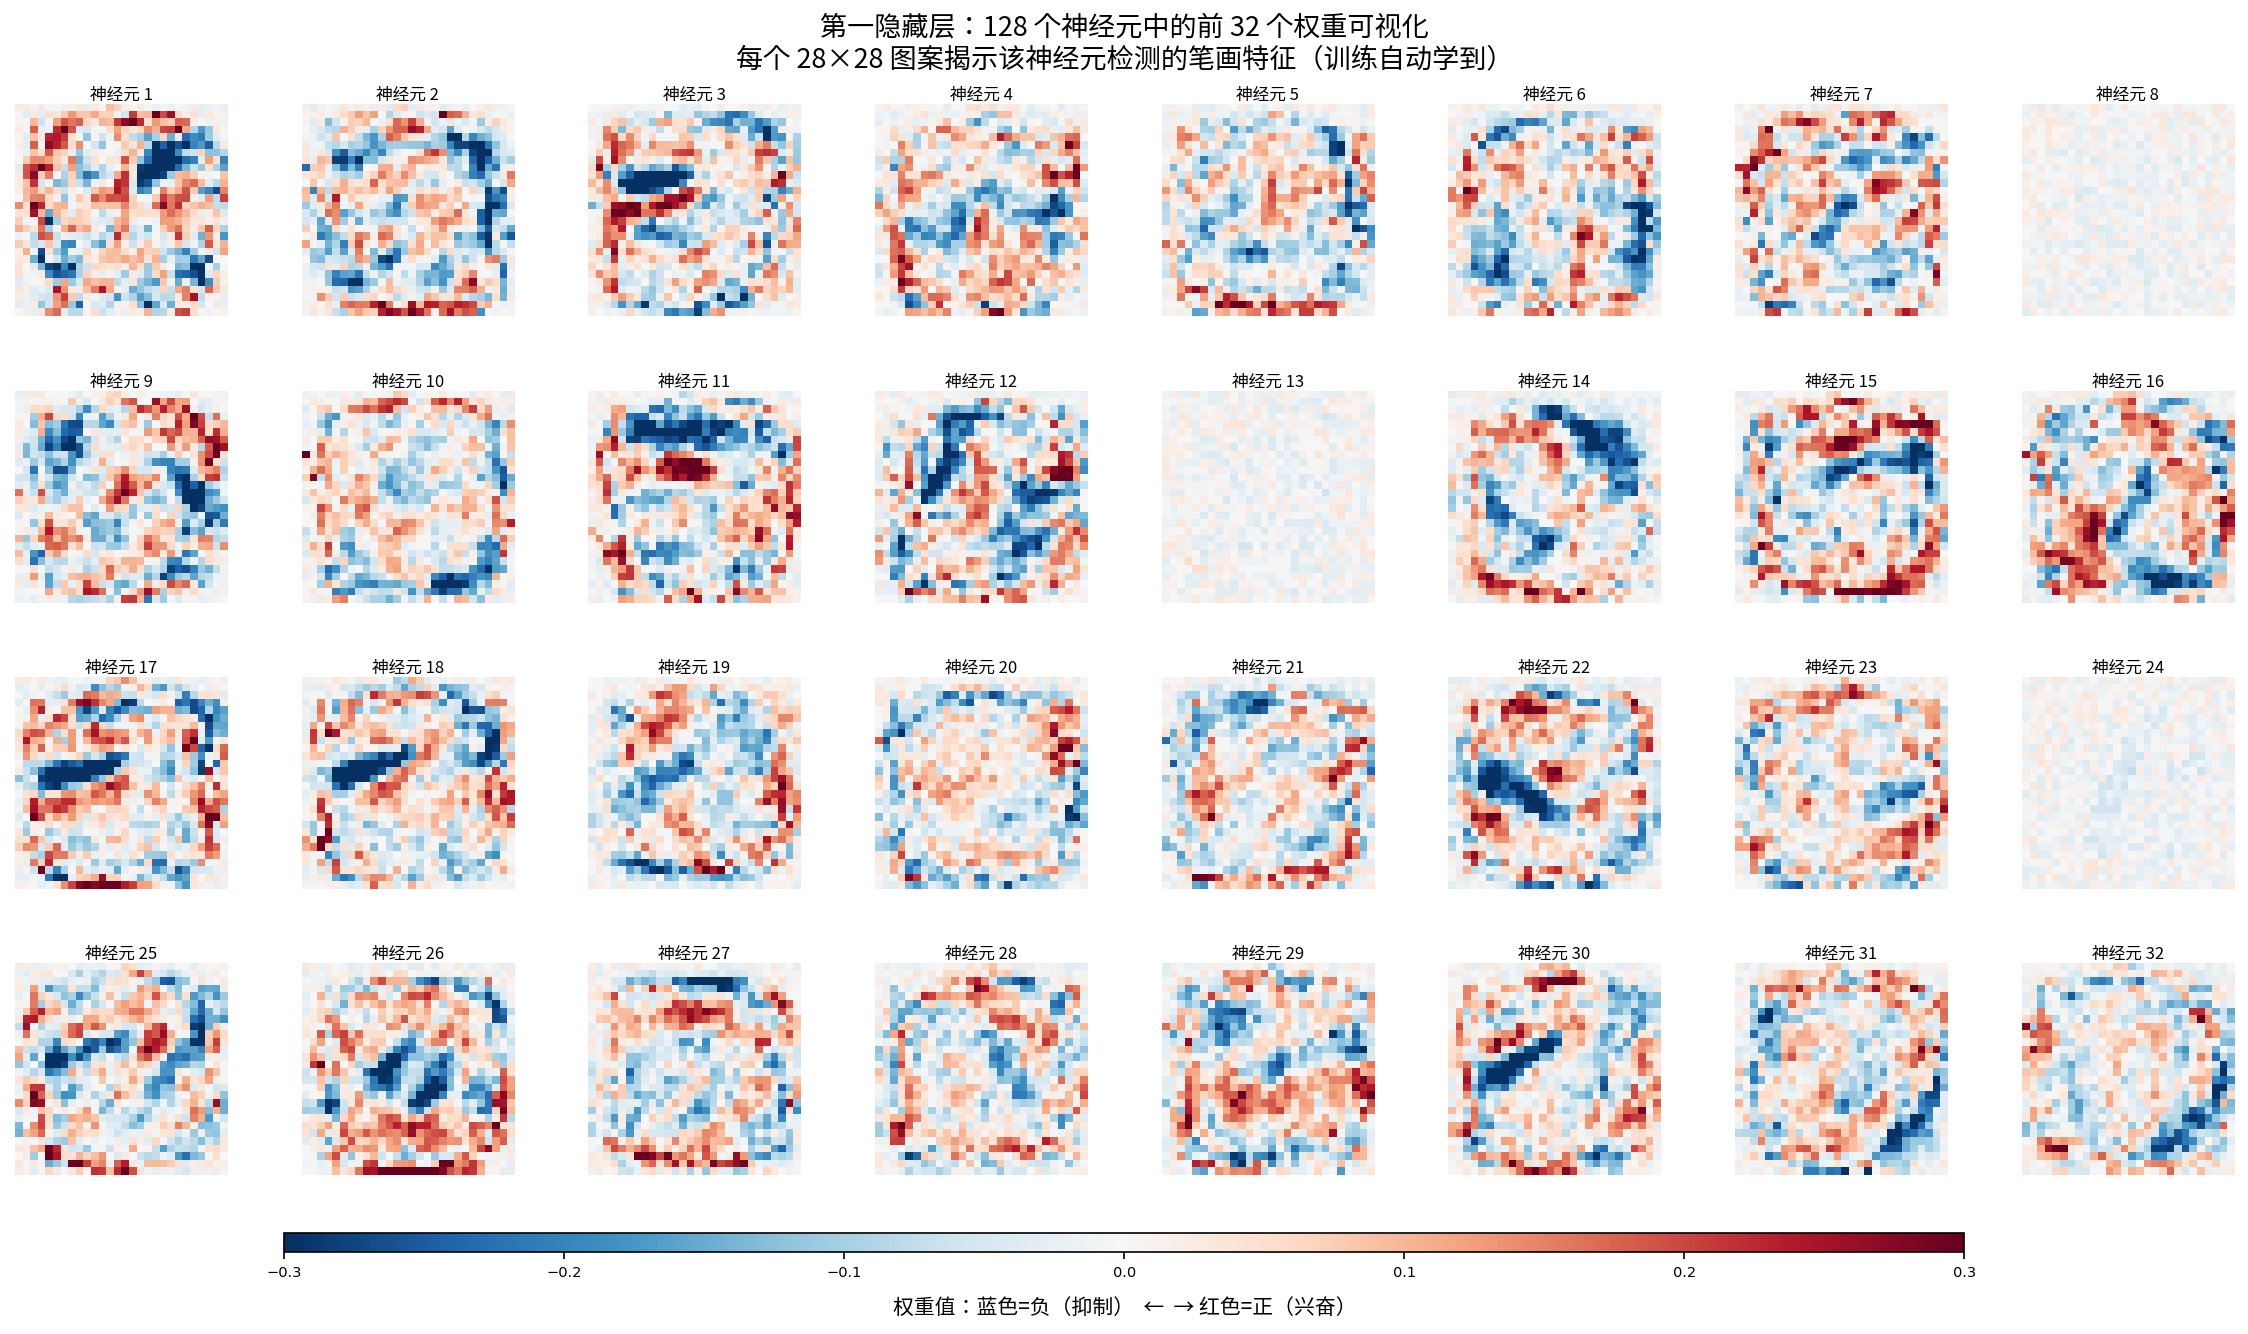
\includegraphics[width=0.7\textwidth]{slide_assets/weight_heatmap.png}
\end{center}

\vspace{0.1cm}

\begin{columns}[T]
\column{0.55\textwidth}
\begin{block}{如何解读这张图？}
\footnotesize
每个 28$\times$28 小图 = 一个神经元的权重 reshape 回 28$\times$28。\\[2pt]
\textbf{红色（正权重）：} 神经元"喜欢"该位置像素值高（兴奋）。\\
\textbf{蓝色（负权重）：} 神经元"不喜欢"该位置像素值高（抑制）。\\[2pt]
\textbf{这些模式是训练自动学到的，不是人为设计。}
\end{block}

\column{0.45\textwidth}
\begin{exampleblock}{关键观察}
\footnotesize
\begin{itemize}
  \item 部分神经元检测横线、竖线、弧线等笔画
  \item 部分神经元抑制背景噪声
  \item 不同神经元分工检测不同特征
\end{itemize}
\textbf{来源：}\texttt{checkpoints/mnist\_mlp.pt}\\
\texttt{net.1.weight}（形状 128$\times$784）
\end{exampleblock}
\end{columns}
\end{frame}

% ═══════════ 14 — 实验结果 + 训练曲线 ═══════════
\begin{frame}[fragile,shrink=10]{实验结果：MLP 在 MNIST 上表现如何}
\small

\begin{columns}[T]
\column{0.5\textwidth}
\begin{center}
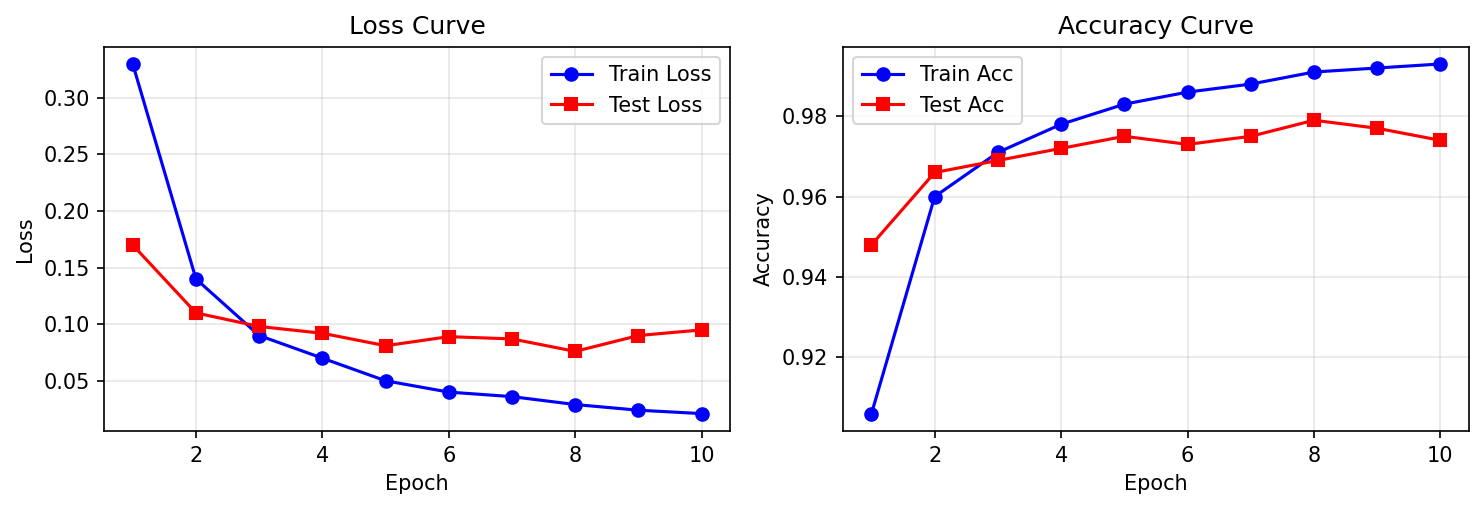
\includegraphics[width=\textwidth]{slide_assets/training_curves.png}
\end{center}

\column{0.5\textwidth}
\begin{block}{关键数值（10 epochs, \texttt{mnist\_mlp.py} 输出）}
\footnotesize
\begin{tabular}{c c c}
\toprule
\textbf{Epoch} & \textbf{Train Acc} & \textbf{Test Acc} \\
\midrule
1  & 90.63\% & 94.81\% \\
5  & 98.26\% & 97.54\% \\
10 & \textbf{99.31\%} & \textbf{97.44\%} \\
\bottomrule
\end{tabular}
\end{block}

\vspace{0.15cm}

\begin{exampleblock}{从曲线中观察}
\footnotesize
\begin{itemize}
  \item Loss 持续下降 $\to$ 模型在学习（\texttt{train\_one\_epoch} 在工作）
  \item 后期测试 Loss 不再下降（甚至微升）$\to$ \textbf{可能开始过拟合}
  \item 训练 Acc 99.3\% vs 测试 Acc 97.4\% $\to$ 约 2\% 泛化差距
  \item 这表明：在 MNIST 上表现好 $\neq$ 模型真正"理解"了图像
  \item 换成 Fashion-MNIST，MLP 的准确率会明显下降（阶段 4 会验证）
\end{itemize}
\end{exampleblock}
\end{columns}

\vspace{0.15cm}
\footnotesize
\textbf{运行命令：} \texttt{conda run -n Teaching python mnist\_mlp.py}\\
\textbf{产出：} \texttt{checkpoints/mnist\_mlp.pt}（109,386 个参数，可用于 C 语言推理）
\end{frame}

% ═══════════ 15 — utils.py ═══════════
\begin{frame}[fragile,shrink=15]{\texttt{utils.py}：支撑整个训练流程的四个工具函数}
\footnotesize

\begin{columns}[T]
\column{0.48\textwidth}
\begin{block}{\texttt{get\_device()} — 自动选 GPU/CPU}
\begin{lstlisting}[basicstyle=\ttfamily\footnotesize, frame=none, numbers=none, backgroundcolor=\color{codebg}]
def get_device():
    return torch.device(
      "cuda" if torch.cuda.is_available()
      else "cpu")
\end{lstlisting}
模型和数据必须在同一设备上。
\end{block}

\vspace{0.1cm}

\begin{block}{\texttt{set\_seed(42)} — 可复现性}
\begin{lstlisting}[basicstyle=\ttfamily\footnotesize, frame=none, numbers=none, backgroundcolor=\color{codebg}]
random.seed(seed)
np.random.seed(seed)
torch.manual_seed(seed)
torch.cuda.manual_seed_all(seed)
\end{lstlisting}
固定所有随机源，保证结果可复现。
\end{block}

\column{0.52\textwidth}
\begin{block}{\texttt{accuracy()} — 分类准确率}
\begin{lstlisting}[basicstyle=\ttfamily\footnotesize, frame=none, numbers=none, backgroundcolor=\color{codebg}]
def accuracy(logits, targets):
    preds = logits.argmax(dim=1)
    return (preds == targets
           ).float().mean().item()
\end{lstlisting}
\texttt{argmax(dim=1)} 取每行最大值的位置作为预测类别。
\end{block}

\vspace{0.1cm}

\begin{block}{\texttt{save\_checkpoint()} — 保存模型}
\begin{lstlisting}[basicstyle=\ttfamily\footnotesize, frame=none, numbers=none, backgroundcolor=\color{codebg}]
def save_checkpoint(model, path):
    torch.save(model.state_dict(), path)
\end{lstlisting}
只保存 \texttt{state\_dict}（权重+偏置），不含模型结构代码。训练好的参数可被 C/Rust/JS 等任何语言读取做推理。
\end{block}
\end{columns}
\end{frame}

% ═══════════ 16 — 模型参数 + 总结 ═══════════
\begin{frame}[shrink=15]{总结：模型参数 + 完整流程回顾}
\small

\begin{columns}[T]
\column{0.45\textwidth}
\begin{block}{训练后的产出：6 个张量}
\footnotesize
\texttt{checkpoints/mnist\_mlp.pt} 包含：
\begin{center}
\begin{tabular}{l l r}
\toprule
\textbf{参数名} & \textbf{形状} & \textbf{元素数} \\
\midrule
\texttt{net.1.weight} & (128, 784) & 100,352 \\
\texttt{net.1.bias}   & (128,)     & 128 \\
\texttt{net.3.weight} & (64, 128)  & 8,192 \\
\texttt{net.3.bias}   & (64,)      & 64 \\
\texttt{net.5.weight} & (10, 64)   & 640 \\
\texttt{net.5.bias}   & (10,)      & 10 \\
\bottomrule
\end{tabular}
\end{center}
\textbf{模型 = 结构（代码） + 参数（数值）}
\end{block}

\column{0.55\textwidth}
\begin{block}{完整流程：4 个文件如何协作}
\footnotesize
\begin{center}
\begin{tikzpicture}[
  node distance=0.4cm and 0.5cm,
  box/.style={draw, rounded corners, minimum width=2.6cm, minimum height=0.6cm,
              align=center, font=\footnotesize},
  arrow/.style={->, >=stealth, thick, mainblue}
]
  \node[box, fill=lightblue!30] (d) {\texttt{data.py}\\加载 MNIST};
  \node[box, fill=lightblue!45, right=of d] (m) {\texttt{models.py}\\MLP 结构};
  \node[box, fill=lightblue!60, right=of m] (u) {\texttt{utils.py}\\工具函数};
  \node[box, fill=greenaccent!25, below=of m] (t) {\texttt{mnist\_mlp.py}\\训练 + 测试};
  \node[box, fill=greenaccent!40, right=of t] (p) {\texttt{checkpoints/}\\mlp.pt 参数};
  \draw[arrow] (d) -- (t);
  \draw[arrow] (m) -- (t);
  \draw[arrow] (u) -- (t);
  \draw[arrow] (t) -- (p);
\end{tikzpicture}
\end{center}

\vspace{0.15cm}

\textbf{本实验覆盖的概念：}\\[2pt]
\begin{tabular}{lll}
\toprule
\textbf{数据} & \textbf{模型} & \textbf{训练} \\
\midrule
Tensor / DataLoader & Linear（全连接） & 前向传播 \\
ToTensor 归一化   & ReLU（激活函数） & 反向传播 \\
batch / shuffle    & Softmax（概率化） & 梯度下降 (Adam) \\
训练集 vs 测试集   & 权重与偏置      & Mini-batch GD \\
\bottomrule
\end{tabular}
\end{block}
\end{columns}

\vspace{0.15cm}

\begin{alertblock}{下一步}
\footnotesize
\textbf{阶段 3：参数导出与 C 语言推理} —— 将 \texttt{state\_dict} 中的 6 个张量导出为文本，在 C 中实现矩阵乘法 + ReLU + argmax，打通 Python 训练 $\to$ 跨语言推理的全流程。\\
\textbf{阶段 4：泛化} —— 换用 Fashion-MNIST/KMNIST/CIFAR-10，同一个模型在不同数据分布上表现如何？
\end{alertblock}
\end{frame}

% ═══════════════════════════════════════════════════════════════
%  阶段 2：CNN — 卷积神经网络
% ═══════════════════════════════════════════════════════════════

% ── 2.1 MLP 的局限 ──
\begin{frame}[shrink=10]{为什么 MLP 不够？——它丢弃了图像的空间结构}
\small

\begin{columns}[T]
\column{0.45\textwidth}
\begin{block}{MLP 的问题}
\footnotesize
\texttt{nn.Flatten()} 把 28$\times$28 图像 "拉直" 为 784 维向量。

\textbf{后果：}
\begin{itemize}
  \item 相邻像素和远距离像素被同等对待
  \item 左上角像素和右下角像素对第一个隐层神经元来说 \\ "距离一样远"
  \item 模型需要\textbf{浪费参数}去重新"发现"哪些像素是邻居
\end{itemize}

\begin{center}
\begin{tikzpicture}[scale=0.6]
  \fill[lightblue!20] (0,0) rectangle (3,3);
  \draw[step=0.5, gray] (0,0) grid (3,3);
  \draw[->, thick, redaccent] (3.3,1.5) -- (4.5,1.5);
  \fill[lightblue!50] (4.8,0.2) rectangle (7.5,2.8);
  \node at (6.15,1.5) {\small 784 维};
  \node at (1.5,-0.5) {28$\times$28 图像};
  \draw[redaccent, thick] (0.25,1.25) rectangle (0.75,1.75);
  \draw[redaccent, thick] (2.25,1.25) rectangle (2.75,1.75);
  \draw[redaccent, thick, dashed] (1.5,5.2) -- (1.5,3);
\end{tikzpicture}
\end{center}
\end{block}

\column{0.55\textwidth}
\begin{block}{CNN 的答案：保留二维结构}
\footnotesize
\textbf{核心思想：} 图像中相邻的像素是相关的——笔画、边缘、纹理都是局部模式。

CNN 用\textbf{卷积核} (convolution kernel) 在图像上滑动，每次只看一个局部窗口。同一个核在整张图上共享参数。

\vspace{0.15cm}
\textbf{两个关键创新：}
\begin{enumerate}
  \item \textbf{局部感受野 (Local Receptive Field):}\\
  每个神经元只看一小块区域（如 3$\times$3），而非全部 784 个像素
  \item \textbf{权重共享 (Weight Sharing):}\\
  同一个 3$\times$3 卷积核滑过整张图，参数量与图像尺寸无关
\end{enumerate}

\vspace{0.15cm}
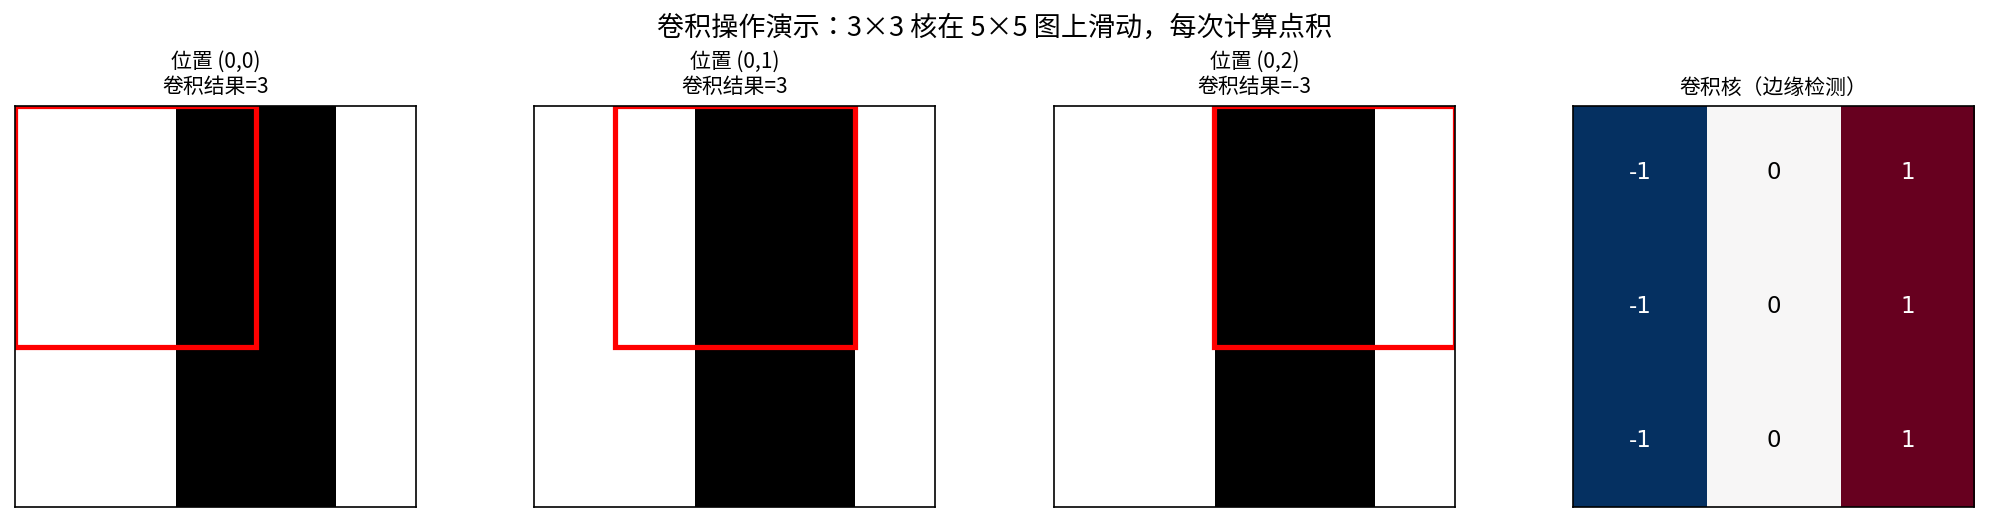
\includegraphics[width=\textwidth]{slide_assets/conv_demo.png}
\end{block}
\end{columns}
\end{frame}

% ── 2.2 卷积操作直观 ──
\begin{frame}[shrink=10]{卷积操作：一个会 "滑动" 的特征检测器}
\small

\begin{columns}[T]
\column{0.48\textwidth}
\begin{center}
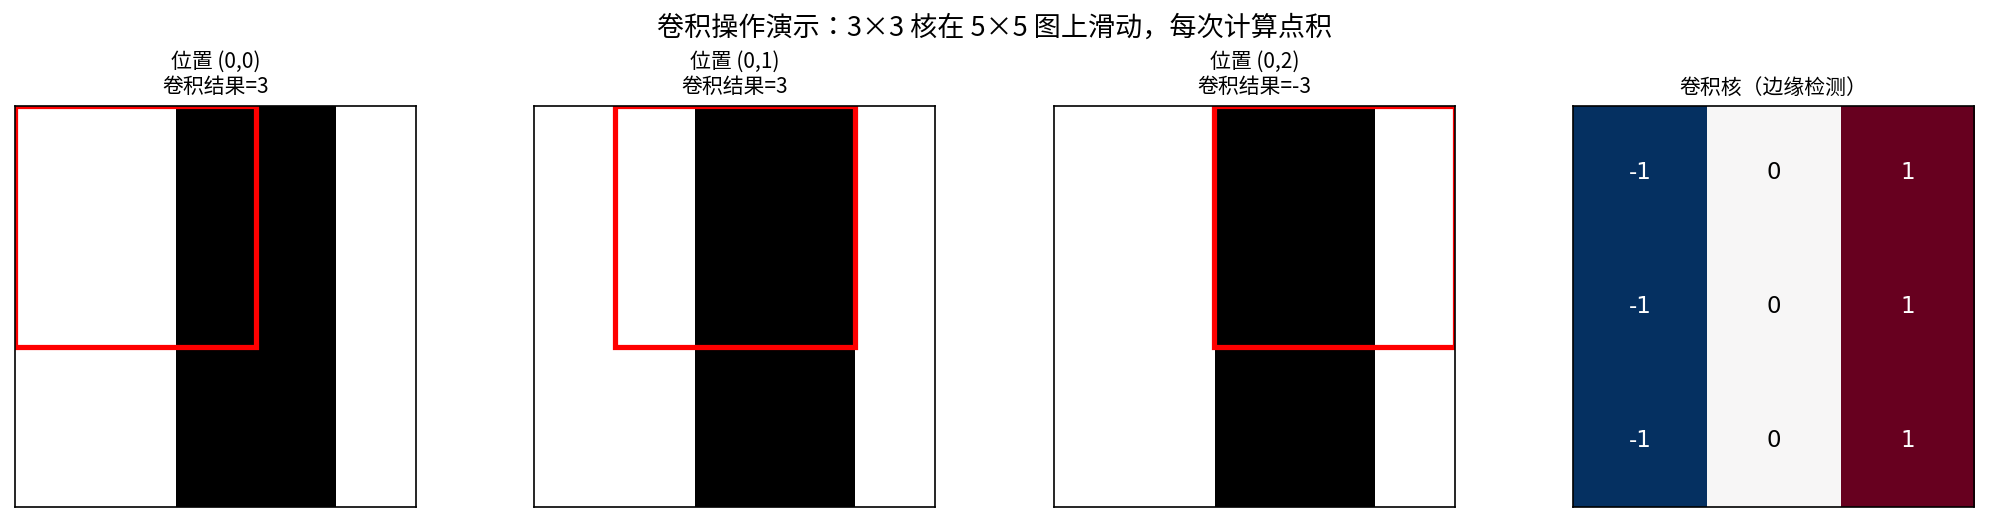
\includegraphics[width=\textwidth]{slide_assets/conv_demo.png}
\end{center}

\column{0.52\textwidth}
\begin{block}{卷积 = 点积 + 滑动}
\footnotesize
\[
\text{output}[i,j] = \sum_{r=0}^{2}\sum_{c=0}^{2} \text{kernel}[r,c] \cdot \text{input}[i+r, j+c]
\]

\textbf{直观理解：}
\begin{itemize}
  \item 卷积核 = 一个 "模板" 或 "特征检测器"
  \item 在图像上逐位置滑动，每步计算核与图像局部区域的相似度
  \item 相似度高 $\to$ 输出大（该位置匹配这个模式）
  \item 相似度低 $\to$ 输出小（该位置不匹配）
\end{itemize}
\end{block}

\vspace{0.15cm}

\begin{exampleblock}{例子：垂直边缘检测核}
\footnotesize
左图卷积核 $\begin{bmatrix}-1&0&1\\-1&0&1\\-1&0&1\end{bmatrix}$ 在图像中间（有竖线的地方）输出大，在平坦区域输出小。\\[2pt]
\textbf{训练时，这些核的数值是自动学到的——不需要人工设计！}
\end{exampleblock}
\end{columns}
\end{frame}

% ── 2.3 Max Pooling ──
\begin{frame}[fragile,shrink=10]{Max Pooling（最大池化）：压缩信息、增强鲁棒性}
\small

\begin{columns}[T]
\column{0.45\textwidth}
\begin{block}{MaxPool2d(2) 做了什么？}
\footnotesize
把特征图划分为 2$\times$2 的小块，每块只保留最大值。

\begin{center}
\begin{tikzpicture}[scale=0.9]
  % 4x4 input
  \fill[lightblue!20] (0,0) rectangle (4,4);
  \draw[step=1, gray] (0,0) grid (4,4);
  \node at (0.5,3.5) {3}; \node at (1.5,3.5) {1};
  \node at (2.5,3.5) {2}; \node at (3.5,3.5) {0};
  \node at (0.5,2.5) {0}; \node at (1.5,2.5) {5};
  \node at (2.5,2.5) {1}; \node at (3.5,2.5) {4};
  \node at (0.5,1.5) {2}; \node at (1.5,1.5) {1};
  \node at (2.5,1.5) {6}; \node at (3.5,1.5) {2};
  \node at (0.5,0.5) {1}; \node at (1.5,0.5) {0};
  \node at (2.5,0.5) {3}; \node at (3.5,0.5) {1};
  \node at (2,-0.3) {4$\times$4 输入};

  \draw[->, thick, mainblue] (4.3,2) -- (5.3,2);

  % 2x2 output
  \fill[lightblue!40] (5.5,1) rectangle (7.5,3);
  \draw[step=1, gray] (5.5,1) grid (7.5,3);
  \node at (6,2.5) {\textbf{5}}; \node at (7,2.5) {\textbf{4}};
  \node at (6,1.5) {\textbf{2}}; \node at (7,1.5) {\textbf{6}};
  \node at (6.5,0.7) {2$\times$2 输出};

  \draw[redaccent, thick] (0,2) rectangle (2,4);
  \draw[redaccent, thick] (5.5,2) rectangle (6.5,3);
\end{tikzpicture}
\end{center}
\end{block}

\column{0.55\textwidth}
\begin{block}{为什么用 MaxPool？}
\footnotesize
\textbf{三个作用：}
\begin{enumerate}
  \item \textbf{降采样：} 尺寸减半（28$\to$14$\to$7），减少计算量
  \item \textbf{增大感受野：} 后续层能看到更大的图像区域
  \item \textbf{平移不变性：} 图像稍微平移，最大值通常还在窗口内
\end{enumerate}

\vspace{0.15cm}
\textbf{在我们的 CNN 中（\texttt{models.py}）：}
\begin{lstlisting}[basicstyle=\ttfamily\footnotesize, frame=none, numbers=none, backgroundcolor=\color{codebg}]
nn.Conv2d(1, 16, 3, padding=1),  # 28x28
nn.ReLU(),
nn.MaxPool2d(2),                 # -> 14x14
nn.Conv2d(16, 32, 3, padding=1), # 14x14
nn.ReLU(),
nn.MaxPool2d(2),                 # -> 7x7
\end{lstlisting}
\end{block}

\vspace{0.15cm}
\footnotesize
\textbf{Padding=1 的作用：} 在图像边缘补一圈 0，使卷积后尺寸不变（28$\times$28 $\to$ 28$\times$28）。\\
不用 padding 的话，3$\times$3 卷积会使尺寸缩小 2 像素（28$\to$26）。
\end{columns}
\end{frame}

% ── 2.4 CNN 结构 + 代码 ──
\begin{frame}[fragile,shrink=15]{CNN 网络结构：\texttt{models.py} 中的 \texttt{CNNClassifier}}
\small

\begin{columns}[T]
\column{0.48\textwidth}
\begin{center}
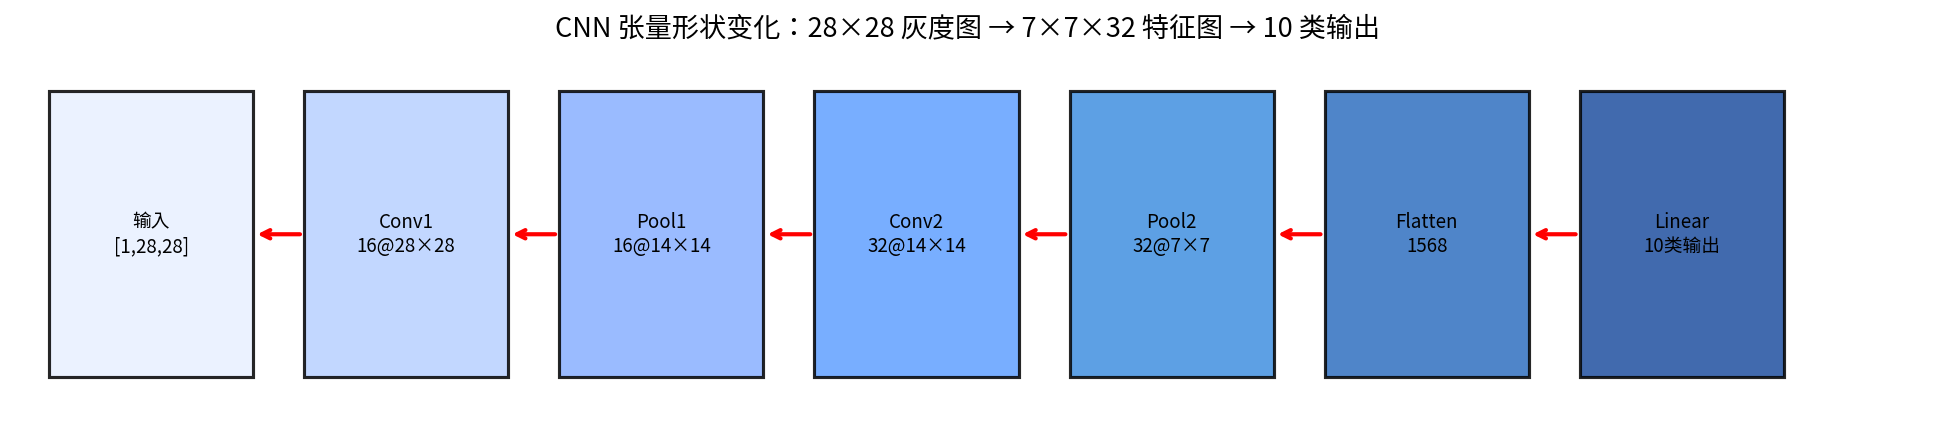
\includegraphics[width=\textwidth]{slide_assets/cnn_shapes.png}
\end{center}

\begin{block}{张量形状流转}
\footnotesize
\centering
\texttt{[1,28,28]} $\to$ Conv1 $\to$ \texttt{[16,28,28]} $\to$ Pool $\to$ \texttt{[16,14,14]}\\
$\to$ Conv2 $\to$ \texttt{[32,14,14]} $\to$ Pool $\to$ \texttt{[32,7,7]}\\
$\to$ Flatten $\to$ \texttt{[1568]} $\to$ Linear $\to$ \texttt{[10]}
\end{block}

\column{0.52\textwidth}
\begin{block}{\texttt{models.py} — CNNClassifier}
\footnotesize
\begin{lstlisting}[basicstyle=\ttfamily\scriptsize, frame=none, numbers=none, backgroundcolor=\color{codebg}]
class CNNClassifier(nn.Module):
    def __init__(self):
        super().__init__()
        self.net = nn.Sequential(
            nn.Conv2d(1,16,3,padding=1),
            nn.ReLU(),
            nn.MaxPool2d(2),        # 14x14
            nn.Conv2d(16,32,3,padding=1),
            nn.ReLU(),
            nn.MaxPool2d(2),        # 7x7
            nn.Flatten(),           # 1568
            nn.Linear(1568, 10),
        )
\end{lstlisting}
\end{block}

\vspace{0.1cm}
\footnotesize
\textbf{参数量：} Conv1: $1\times16\times9+16=160$, Conv2: $16\times32\times9+32=4{,}640$, Linear: $1568\times10+10=15{,}690$, \textbf{总计: 20,490}（vs MLP 109,386）
\end{columns}
\end{frame}

% ── 2.5 卷积核可视化 ──
\begin{frame}[shrink=25]{卷积核可视化：CNN 第一层学到了什么？}
\small

\begin{center}
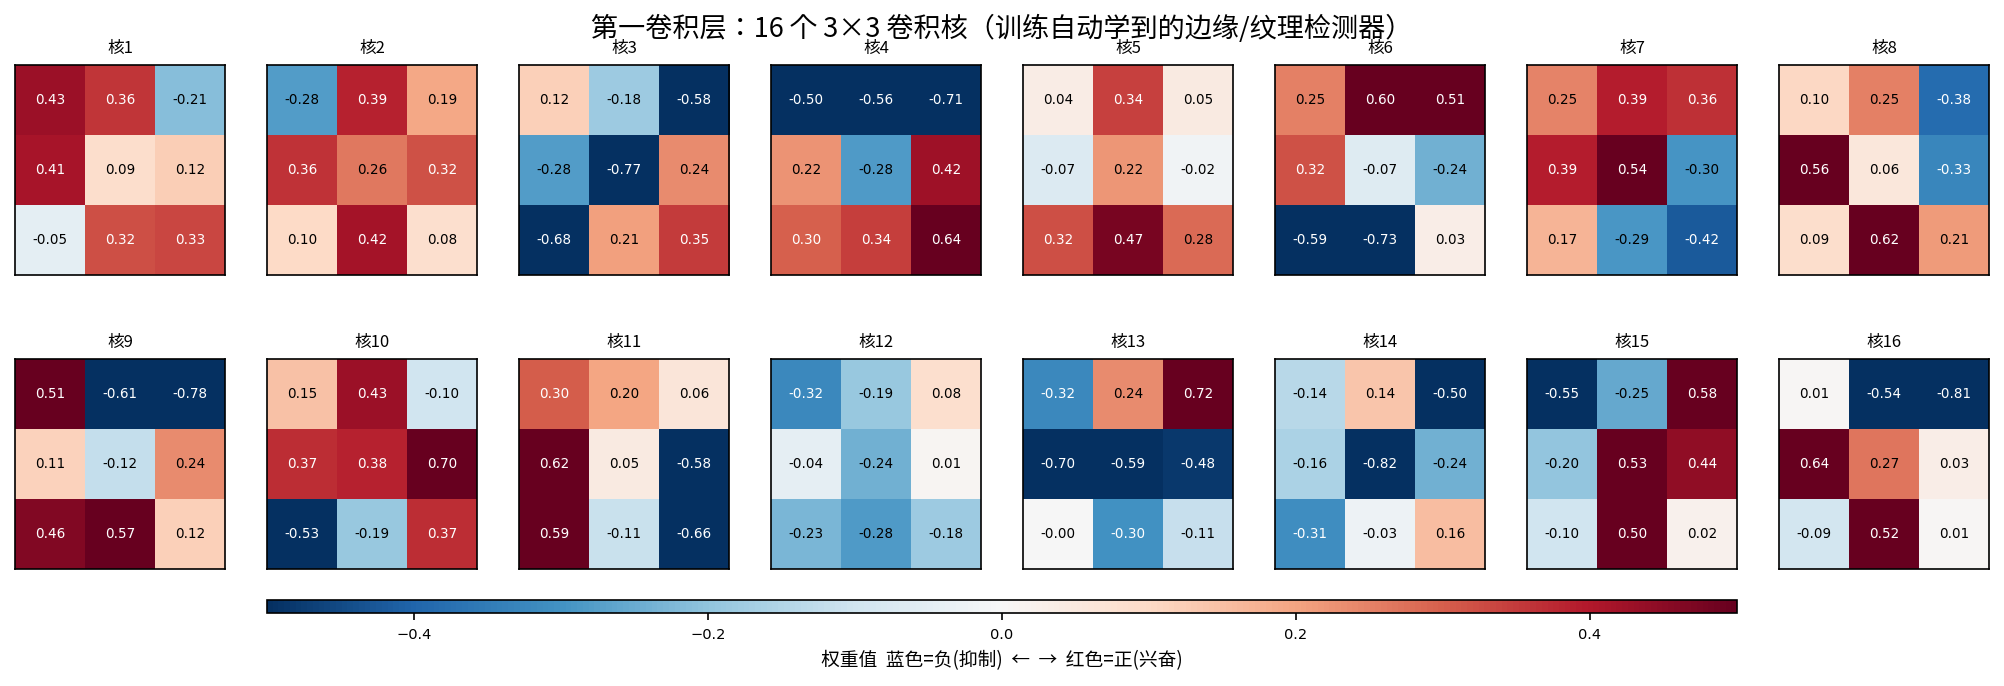
\includegraphics[width=0.68\textwidth]{slide_assets/cnn_kernels.png}
\end{center}

\vspace{-0.1cm}

\begin{columns}[T]
\column{0.48\textwidth}
\begin{block}{如何解读？}
\footnotesize
每个 3$\times$3 小图是一个卷积核。\textbf{红色=正，蓝色=负。}\\
检测\textbf{局部边缘和纹理}：水平边缘、垂直边缘、对角线或斑点。\\[1pt]
与 MLP 第一层 784 维权重不同——3$\times$3 核\textbf{直观可解释}。
\end{block}

\column{0.52\textwidth}
\begin{exampleblock}{CNN 的核心优势}
\footnotesize
\begin{itemize}
  \item 卷积核 = 局部特征模板，\textbf{人眼可理解}
  \item 16 个核各司其职：检测不同方向的边缘
  \item 权重共享：同一核滑过全图，与位置无关
  \item 参数少 + 可解释 + 效果更好
\end{itemize}
\end{exampleblock}
\end{columns}
\end{frame}

% ── 2.6 MLP vs CNN 对比 ──
\begin{frame}[shrink=15]{MLP vs CNN：全面对比}
\small

\begin{center}
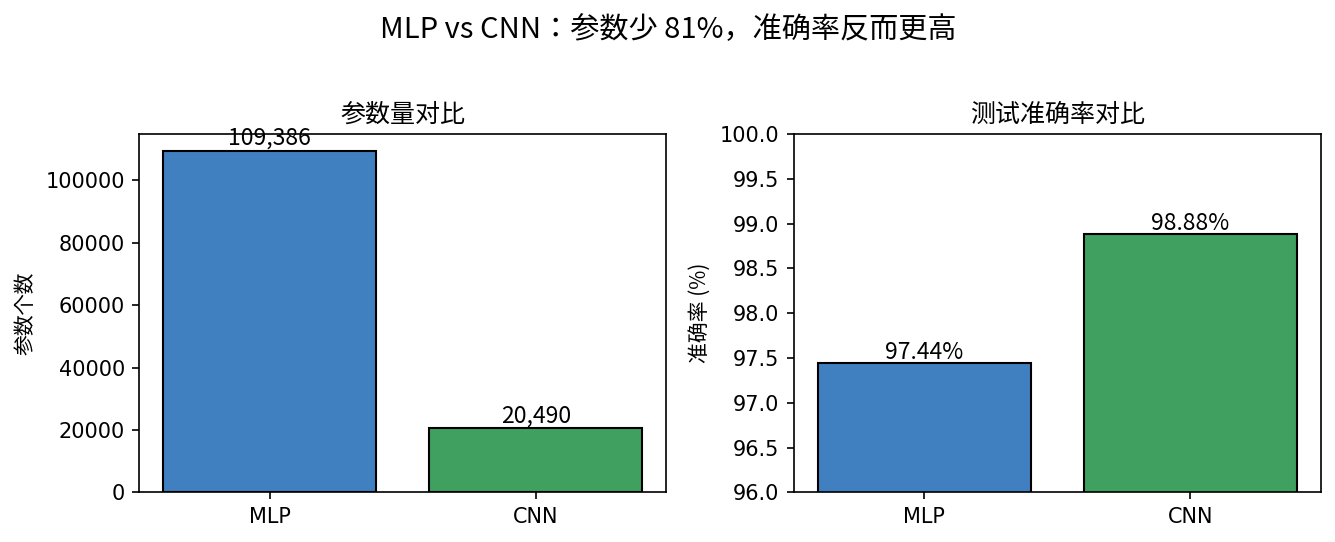
\includegraphics[width=0.65\textwidth]{slide_assets/mlp_cnn_compare.png}
\end{center}

\vspace{0.05cm}

\begin{columns}[T]
\column{0.333\textwidth}
\begin{block}{参数量}
\footnotesize
\centering
MLP: \textbf{109,386}\\[1pt]
CNN: \textbf{20,490}\\[2pt]
CNN 仅 MLP 的 \textbf{19\%}\\
权重共享大幅降参
\end{block}

\column{0.333\textwidth}
\begin{block}{测试准确率}
\footnotesize
\centering
MLP: \textbf{97.44\%}\\[1pt]
CNN: \textbf{98.88\%}\\[2pt]
参数少 81\%\\
准确率\textbf{反高 1.44\%}
\end{block}

\column{0.334\textwidth}
\begin{block}{收敛速度}
\footnotesize
\centering
MLP E1: 94.81\%\\[1pt]
CNN E1: \textbf{97.55\%}\\[2pt]
CNN 第 1 轮即逼近\\
MLP 最终水平\\
卷积\textbf{归纳偏置}天然适合图像
\end{block}
\end{columns}

\vspace{0.1cm}
\footnotesize
\begin{center}
\textbf{核心原因：CNN 的卷积结构利用了图像的二维局部性——MLP 的 Flatten 操作完全丢弃了这些信息。}
\end{center}
\end{frame}

% ═══════════════════════════════════════════════════════════════
%  阶段 3：参数导出与 C 语言推理
% ═══════════════════════════════════════════════════════════════

% ── 3.1 训练 vs 推理 ──
\begin{frame}[shrink=10]{训练 vs 推理：同一个模型，两种运行模式}
\small

\begin{columns}[T]
\column{0.48\textwidth}
\begin{block}{训练 (Training)}
\footnotesize
\begin{center}
\begin{tikzpicture}[node distance=0.4cm]
  \node[draw, rounded corners, fill=lightblue!40, minimum width=2.5cm, minimum height=0.6cm] (a) {前向传播};
  \node[draw, rounded corners, fill=lightblue!50, right=of a, minimum width=2.5cm, minimum height=0.6cm] (b) {计算损失};
  \node[draw, rounded corners, fill=redaccent!20, below=of a, minimum width=2.5cm, minimum height=0.6cm] (c) {反向传播};
  \node[draw, rounded corners, fill=redaccent!30, right=of c, minimum width=2.5cm, minimum height=0.6cm] (d) {更新参数};
  \draw[->, thick] (a) -- (b);
  \draw[->, thick] (b) -- (d);
  \draw[->, thick] (d) -- (c);
  \draw[->, thick] (c) -- (a);
\end{tikzpicture}
\end{center}
\vspace{0.1cm}
需要：数据 + 标签 + 损失函数 + 优化器 + 梯度计算

\textbf{需要 PyTorch 的 autograd 系统。}
\end{block}

\column{0.52\textwidth}
\begin{block}{推理 (Inference)}
\footnotesize
\begin{center}
\begin{tikzpicture}[node distance=0.4cm]
  \node[draw, rounded corners, fill=greenaccent!20, minimum width=4cm, minimum height=0.7cm] (a) {输入 $\to$ 前向传播 $\to$ 输出};
\end{tikzpicture}
\end{center}
\vspace{0.1cm}
只需要：输入数据 + 固定参数 + 前向计算

\textbf{不需要 PyTorch。不需要 GPU。不需要梯度。}
\end{block}
\end{columns}

\vspace{0.3cm}

\begin{alertblock}{核心认知}
\footnotesize
训练完成后，模型就是\textbf{一组固定的数值参数} + \textbf{一段确定性的前向计算}。

前向计算只涉及四种操作：\textbf{矩阵乘法、向量加法、ReLU、argmax}。\\
这些是任何编程语言都支持的基础数学运算。

$\to$ Python 训练的模型，可以在 C、Rust、JavaScript 甚至嵌入式中运行推理。
\end{alertblock}
\end{frame}

% ── 3.2 参数导出 ──
\begin{frame}[fragile,shrink=25]{参数导出：把 \texttt{.pt} 文件变成可读的文本}
\small

\begin{columns}[T]
\column{0.52\textwidth}
\begin{block}{\texttt{export\_mlp\_params.py} 做了什么？}
\footnotesize
加载 \texttt{checkpoints/mnist\_mlp.pt}，取出 6 个张量，保存为纯文本：

\vspace{-0.1cm}
\begin{center}
\begin{tabular}{l l}
\toprule
\textbf{文件} & \textbf{内容} \\
\midrule
\texttt{params/layer1\_weight.txt} & 128 $\times$ 784 \\
\texttt{params/layer1\_bias.txt}   & 128 个浮点数 \\
\texttt{params/layer2\_weight.txt} & 64 $\times$ 128 \\
\texttt{params/layer2\_bias.txt}   & 64 个浮点数 \\
\texttt{params/layer3\_weight.txt} & 10 $\times$ 64 \\
\texttt{params/layer3\_bias.txt}   & 10 个浮点数 \\
\bottomrule
\end{tabular}
\end{center}
\textbf{为什么用文本格式？} 可人工检查、C 语言 \texttt{fscanf} 直接读、跨平台通用。
\end{block}

\column{0.48\textwidth}
\begin{block}{同时导出测试样本}
\footnotesize
\begin{lstlisting}[basicstyle=\ttfamily\footnotesize, frame=none, numbers=none, backgroundcolor=\color{codebg}]
# samples/sample_0.txt
# MNIST test sample 0, label=7
0.0000 0.0000 ... 0.0000
0.0000 0.0118 ... 0.0000
...
\end{lstlisting}
每张图 28$\times$28 像素，归一化到 [0,1]。\\
标签记录在 \texttt{samples/labels.txt}。
\end{block}

\vspace{0.15cm}

\begin{block}{核心认知}
\footnotesize
\texttt{.pt} 文件 $\to$ 文本文件 $\to$ 任何语言可读。\\
\textbf{训练一次，到处部署。} 这就是模型参数导出的意义。
\end{block}
\end{columns}
\end{frame}

% ── 3.3 C 推理代码 ──
\begin{frame}[fragile,shrink=15]{C 语言推理：\texttt{mnist\_mlp\_infer.c} 核心函数}
\footnotesize

\begin{columns}[T]
\column{0.5\textwidth}
\begin{block}{矩阵乘向量 + 偏置 (\texttt{linear})}
\begin{lstlisting}[basicstyle=\ttfamily\footnotesize, frame=none, numbers=none, backgroundcolor=\color{codebg}]
void linear(float *w, float *x,
            float *b, float *y,
            int out_dim, int in_dim)
{
  for (int i = 0; i < out_dim; i++) {
    float sum = b[i];
    for (int j = 0; j < in_dim; j++)
      sum += w[i*in_dim + j] * x[j];
    y[i] = sum;
  }
}
\end{lstlisting}
这是整个推理的\textbf{计算核心}。\\
两层循环：外层遍历输出神经元，内层做点积。
\end{block}

\column{0.5\textwidth}
\begin{block}{ReLU + Argmax}
\begin{lstlisting}[basicstyle=\ttfamily\footnotesize, frame=none, numbers=none, backgroundcolor=\color{codebg}]
void relu(float *x, int n) {
  for (int i = 0; i < n; i++)
    if (x[i] < 0.0f) x[i] = 0.0f;
}

int argmax(float *x, int n) {
  int best = 0;
  for (int i = 1; i < n; i++)
    if (x[i] > x[best]) best = i;
  return best;
}
\end{lstlisting}
\textbf{ReLU:} 遍历数组，负数置零。一行代码。

\textbf{Argmax:} 遍历数组，找最大值索引。两行代码。
\end{block}
\end{columns}

\vspace{0.15cm}

\begin{block}{完整前向传播（\texttt{main} 函数中）}
\begin{lstlisting}[basicstyle=\ttfamily\small, frame=none, numbers=none, backgroundcolor=\color{codebg}]
linear(w1, input, b1, h1, 128, 784);  relu(h1, 128);   // 第1层: 784 -> 128
linear(w2, h1,   b2, h2, 64, 128);    relu(h2, 64);    // 第2层: 128 -> 64
linear(w3, h2,   b3, logits, 10, 64);                  // 第3层: 64 -> 10 (无ReLU)
int pred = argmax(logits, 10);                          // 取最大分数为预测类别
\end{lstlisting}
\end{block}
\end{frame}

% ── 3.4 C 推理验证 ──
\begin{frame}[fragile,shrink=10]{验证：C 推理 vs Python 推理 —— 结果完全一致}
\small

\begin{columns}[T]
\column{0.45\textwidth}
\begin{block}{验证方法}
\footnotesize
\begin{enumerate}
  \item Python \texttt{export\_mlp\_params.py} 导出参数 + 5 张测试图片
  \item C 程序读取参数和图片，做前向传播
  \item Python (numpy) 用同样参数做前向传播
  \item 比较两者的 logits 和预测类别
\end{enumerate}
\end{block}

\begin{block}{编译与运行}
\footnotesize
\begin{lstlisting}[basicstyle=\ttfamily\footnotesize, frame=none, numbers=none, backgroundcolor=\color{codebg}]
$ gcc -o mnist_mlp_infer \
    mnist_mlp_infer.c -lm
$ ./mnist_mlp_infer \
    samples/sample_0.txt
Prediction: 7
\end{lstlisting}
\end{block}

\column{0.55\textwidth}
\begin{block}{5 个样本验证结果}
\footnotesize
\begin{center}
\begin{tabular}{c c c c}
\toprule
\textbf{样本} & \textbf{真实标签} & \textbf{C 预测} & \textbf{结果} \\
\midrule
sample\_0 & 7 & 7 & OK \\
sample\_1 & 2 & 2 & OK \\
sample\_2 & 1 & 1 & OK \\
sample\_3 & 0 & 0 & OK \\
sample\_4 & 4 & 4 & OK \\
\bottomrule
\end{tabular}
\end{center}
\textbf{Logits 最大误差：}$8.1 \times 10^{-7}$（浮点精度差异）
\end{block}

\vspace{0.15cm}

\begin{exampleblock}{这意味着什么？}
\footnotesize
\begin{itemize}
  \item 训练好的模型可以\textbf{脱离 Python/PyTorch 环境}独立运行
  \item 推理只需要基础数学运算——任何语言、任何平台都能做
  \item 这就是模型部署的本质：\textbf{训练用框架，推理用基础运算}
  \item CNN 的 C 推理同理：多出 conv2d 和 maxpool2d，但仍只是数值计算
\end{itemize}
\end{exampleblock}
\end{columns}
\end{frame}

% ── 3.5 总结：三阶段全景 ──
\begin{frame}[shrink=15]{三阶段全景回顾}
\small

\begin{center}
\begin{tikzpicture}[
  node distance=0.5cm and 1.2cm,
  stage/.style={draw, rounded corners, minimum width=4cm, minimum height=1.3cm,
                align=center, font=\small},
  arrow/.style={->, >=stealth, ultra thick, mainblue}
]
  \node[stage, fill=lightblue!30] (s1) {\textbf{阶段 1: MLP 基线}\\[2pt]
   \footnotesize 784$\to$128$\to$64$\to$10\\109K 参数，97.4\% 准确率};
  \node[stage, fill=lightblue!50, right=of s1] (s2) {\textbf{阶段 2: CNN}\\[2pt]
   \footnotesize Conv$\to$Pool$\to$Conv$\to$Pool$\to$FC\\20K 参数，98.9\% 准确率};
  \node[stage, fill=lightblue!70, right=of s2] (s3) {\textbf{阶段 3: C 推理}\\[2pt]
   \footnotesize 导出参数 $\to$ C 语言前向传播\\5/5 样本与 Python 一致};

  \draw[arrow] (s1) -- (s2);
  \draw[arrow] (s2) -- (s3);
\end{tikzpicture}
\end{center}

\vspace{0.3cm}

\begin{columns}[T]
\column{0.33\textwidth}
\begin{block}{阶段 1 核心收获}
\footnotesize
\begin{itemize}
  \item 数据 $\to$ 模型 $\to$ 训练 $\to$ 测试的完整流程
  \item 前向/反向/梯度下降的含义
  \item Softmax、交叉熵、ReLU 的作用
  \item \texttt{data.py} / \texttt{models.py} / \texttt{utils.py} 可复用骨架
\end{itemize}
\end{block}

\column{0.33\textwidth}
\begin{block}{阶段 2 核心收获}
\footnotesize
\begin{itemize}
  \item CNN 通过卷积保留二维空间结构
  \item 局部感受野 + 权重共享 = 更少参数 + 更好效果
  \item 卷积核可视化：可解释的局部特征
  \item MLP vs CNN：结构决定效率
\end{itemize}
\end{block}

\column{0.34\textwidth}
\begin{block}{阶段 3 核心收获}
\footnotesize
\begin{itemize}
  \item 模型 = 结构（代码）+ 参数（数值）
  \item 推理只需四种运算：矩阵乘、加法、ReLU、argmax
  \item PyTorch 训练的模型可跨语言部署
  \item Python $\to$ C 打通了训练到部署的全链路
\end{itemize}
\end{block}
\end{columns}
\end{frame}

% ═══════════════════════════════════════════════════════════════
%  附录：程序使用指南
% ═══════════════════════════════════════════════════════════════

% ── 程序总览 ──
\begin{frame}[fragile,shrink=15]{配套程序使用指南（一）：训练与推理}
\footnotesize

\begin{columns}[T]
\column{0.5\textwidth}
\begin{block}{\texttt{mnist\_mlp.py} — MLP 训练}
\begin{lstlisting}[basicstyle=\ttfamily\scriptsize, frame=none, numbers=none, backgroundcolor=\color{codebg}]
conda run -n Teaching python mnist_mlp.py
\end{lstlisting}
\vspace{-0.3cm}
\begin{itemize}
  \item 训练三层 MLP（784$\to$128$\to$64$\to$10）
  \item 产出 \texttt{checkpoints/mnist\_mlp.pt}
  \item 测试准确率 $\approx$ 97.4\%，约 1—2 分钟
\end{itemize}
\end{block}

\vspace{0.1cm}

\begin{block}{\texttt{mnist\_cnn.py} — CNN 训练}
\begin{lstlisting}[basicstyle=\ttfamily\scriptsize, frame=none, numbers=none, backgroundcolor=\color{codebg}]
conda run -n Teaching python mnist_cnn.py
\end{lstlisting}
\vspace{-0.3cm}
\begin{itemize}
  \item 训练 CNN（2 层卷积+池化）
  \item 产出 \texttt{checkpoints/mnist\_cnn.pt}
  \item 20K 参数，准确率 $\approx$ 98.9\%，约 2—3 分钟
\end{itemize}
\end{block}

\vspace{0.1cm}

\begin{block}{\texttt{sampling.py} — 手写交互采样}
\begin{lstlisting}[basicstyle=\ttfamily\scriptsize, frame=none, numbers=none, backgroundcolor=\color{codebg}]
conda run -n Teaching python sampling.py
\end{lstlisting}
\vspace{-0.3cm}
\begin{itemize}
  \item 鼠标写数字 $\to$ 28$\times$28 灰度图
  \item 支持实时 MLP 预测（需先训练）
  \item s:保存(png) t:保存(文本) p:预测 c:清空
\end{itemize}
\end{block}

\column{0.5\textwidth}
\begin{block}{\texttt{export\_mlp\_params.py} — 参数导出}
\begin{lstlisting}[basicstyle=\ttfamily\scriptsize, frame=none, numbers=none, backgroundcolor=\color{codebg}]
conda run -n Teaching python export_mlp_params.py
\end{lstlisting}
\vspace{-0.3cm}
\begin{itemize}
  \item 导出 6 个张量为文本文件到 \texttt{params/}
  \item 导出 5 张测试样本到 \texttt{samples/}
  \item 自动验证：numpy vs PyTorch 误差 $<$ 10$^{-6}$
\end{itemize}
\end{block}

\vspace{0.1cm}

\begin{block}{\texttt{mnist\_mlp\_infer.c} — C 语言推理}
\begin{lstlisting}[basicstyle=\ttfamily\scriptsize, frame=none, numbers=none, backgroundcolor=\color{codebg}]
$ gcc -o mnist_mlp_infer mnist_mlp_infer.c -lm
$ ./mnist_mlp_infer samples/sample_0.txt
Prediction: 7
\end{lstlisting}
\vspace{-0.3cm}
\begin{itemize}
  \item 纯 C 实现：矩阵乘 + 加法 + ReLU + argmax
  \item 与 Python 推理结果完全一致
\end{itemize}
\end{block}

\vspace{0.1cm}

\begin{block}{\texttt{download\_datasets.sh} — 下载数据}
\begin{lstlisting}[basicstyle=\ttfamily\scriptsize, frame=none, numbers=none, backgroundcolor=\color{codebg}]
bash download_datasets.sh datasets
\end{lstlisting}
\vspace{-0.3cm}
下载 MNIST / Fashion-MNIST / KMNIST / CIFAR-10。
\end{block}
\end{columns}
\end{frame}

% ── 典型工作流 ──
\begin{frame}[fragile,shrink=10]{配套程序使用指南（二）：典型工作流}
\small

\begin{block}{第一次使用：从头训练}
\footnotesize
\begin{center}
\begin{tikzpicture}[
  node distance=0.4cm,
  wfbox/.style={draw, rounded corners, minimum width=2.8cm, minimum height=0.65cm,
               align=center, font=\footnotesize, fill=lightblue!40},
  arrow/.style={->, >=stealth, thick, mainblue}
]
  \node[wfbox] (a) {下载数据\\\texttt{download\_datasets.sh}};
  \node[wfbox, right=of a] (b) {训练 MLP\\\texttt{mnist\_mlp.py}};
  \node[wfbox, right=of b] (c) {训练 CNN\\\texttt{mnist\_cnn.py}};
  \node[wfbox, below=of c] (d) {导出参数\\\texttt{export\_mlp\_params.py}};
  \node[wfbox, below=of d] (e) {C 推理验证\\\texttt{mnist\_mlp\_infer}};
  \node[wfbox, left=of e] (f) {手写测试\\\texttt{sampling.py}};
  \draw[arrow] (a) -- (b);
  \draw[arrow] (b) -- (c);
  \draw[arrow] (c) -- (d);
  \draw[arrow] (d) -- (e);
  \draw[arrow] (d) -- (f);
\end{tikzpicture}
\end{center}
\end{block}

\vspace{0.15cm}

\begin{columns}[T]
\column{0.48\textwidth}
\begin{block}{模型已训练：快速推理}
\footnotesize
\textbf{Python 推理：}
\begin{lstlisting}[basicstyle=\ttfamily\footnotesize, frame=none, numbers=none, backgroundcolor=\color{codebg}]
import torch
from models import MLPClassifier
model = MLPClassifier()
model.load_state_dict(
  torch.load("checkpoints/mnist_mlp.pt"))
model.eval()
# ... forward pass ...
\end{lstlisting}

\textbf{C 推理：}
\begin{lstlisting}[basicstyle=\ttfamily\footnotesize, frame=none, numbers=none, backgroundcolor=\color{codebg}]
./mnist_mlp_infer samples/drawn_000.txt
\end{lstlisting}
\end{block}

\column{0.52\textwidth}
\begin{exampleblock}{关键文件依赖关系}
\footnotesize
\begin{center}
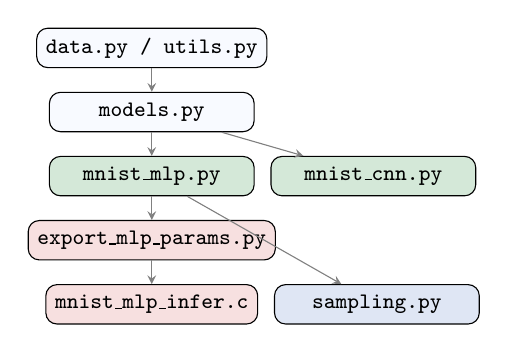
\begin{tikzpicture}[
  node distance=0.3cm and 0.2cm,
  f/.style={draw, rounded corners, font=\footnotesize\ttfamily, minimum width=2.6cm,
            minimum height=0.5cm, align=center, fill=lightblue!30},
  arrow/.style={->, >=stealth, gray}
]
  \node[f] (data) {data.py / utils.py};
  \node[f, below=of data] (models) {models.py};
  \node[f, below=of models, fill=greenaccent!20] (mlp) {mnist\_mlp.py};
  \node[f, right=of mlp, fill=greenaccent!20] (cnn) {mnist\_cnn.py};
  \node[f, below=of mlp, fill=redaccent!15] (exp) {export\_mlp\_params.py};
  \node[f, below=of exp, fill=redaccent!15] (c) {mnist\_mlp\_infer.c};
  \node[f, right=of c, fill=mainblue!15] (samp) {sampling.py};
  \draw[arrow] (data) -- (models);
  \draw[arrow] (models) -- (mlp);
  \draw[arrow] (models) -- (cnn);
  \draw[arrow] (mlp) -- (exp);
  \draw[arrow] (exp) -- (c);
  \draw[arrow] (mlp) -- (samp);
\end{tikzpicture}
\end{center}
\vspace{-0.1cm}
绿色=训练脚本，红色=阶段3（C推理），蓝色=交互测试。
\end{exampleblock}
\end{columns}
\end{frame}

\end{document}
